% !TeX root = main.tex

\documentclass[openright,twoside,headsepline,bibliography=totoc]{scrbook}
% The document is a book with a few options:
%   openright: a new chapter is always on the right page
%   twoside: left and right margins are inverted for even and odd pages

% == Packages and some options
\usepackage{amssymb,amsmath}
\usepackage{ifxetex,ifluatex}
\usepackage{fix-cm}
\usepackage{microtype}  % better justifications, amongst others
\usepackage{longtable,booktabs}

% Make hyperref silent, it's always complaining for tokens like \beta
\usepackage{silence}
%\WarningFilter*{hyperref}{Token not allowed in a PDF string (Unicode)}

\usepackage[unicode=true,pdfa]{hyperref}
\hypersetup{breaklinks=true,
            pdfauthor={Maël Le Garrec},
            pdftitle={LHC Effective Model for Optics Corrections},
            colorlinks=true,
            citecolor=blue,
            urlcolor=blue,
            linkcolor=black,
            pdfborder={0 0 0}}
\usepackage[capitalise]{cleveref}
\usepackage[english]{babel}

% == FONTS
\usepackage{calligra}  % font for quote page
%\usepackage{libertinust1math}
\usepackage{libertine}  % font for the whole document
\usepackage[libertine]{newtxmath}
%\usepackage{lmodern}  % font based on Computer Modern for the whole doc
% ==


\usepackage{wasysym}
\usepackage{enumitem}  % to define new lists
\usepackage{tikz}  % for drawing figures by code
\usepackage{siunitx}
\usepackage{graphicx}
\usepackage{caption}
\usepackage{ragged2e}
\usepackage{atveryend}
%\usepackage{subfigure} (???)
\usepackage{subcaption}
\usepackage{pgf}  % fileformat for the flipbook
\usepackage{xcolor,soul}
\usepackage{lscape}  % landscape
\usepackage{changepage}
\usepackage[nonumberlist,acronyms,nogroupskip]{glossaries}
\usepackage{glossary-longbooktabs}
\usepackage{setspace}
\usepackage[english]{babel}
\usepackage{float}
%\usepackage[subfigure]{tocloft}
\usepackage{titletoc}
\usepackage{etoc}  % local tables of content
\usepackage{imakeidx}
\usepackage{lipsum}
\usepackage{geometry}
\usepackage[automark]{scrlayer-scrpage} % for headers and footers
\usepackage{scrhack}  % to remove some warnings
\usepackage{blindtext}
%\usepackage{unicode-math} % Setup an unicode font for regular typing and for maths  // clashes with OverBrace from nicematrix
\usepackage{amsmath}
\usepackage{mathtools}  % for some functions, like DeclarePairedDelimiter
\usepackage{svg}
\usepackage{nicematrix}
\usepackage[
  height={2cm},
  topthumbmargin={auto},
  bottomthumbmargin={auto},
  eventxtindent={4mm},
  oddtxtexdent={2.5mm}]{thumbs}  % markers on the side to show the chapter
\usepackage[%
  backend=bibtex        % biber or bibtex
%,style=authoryear      % Alphabeticalsch
 ,style=numeric-comp    % numerical-compressed
 ,sorting=none          % no sorting
 ,sortcites=true        % some other example options ...
 ,block=none
 ,indexing=false
 ,citereset=none
 ,isbn=false
 ,url=true
 ,doi=true              % prints doi
 ,natbib=true           % if you need natbib functions
]{biblatex}
\AtEveryBibitem{%  % in the bibliography
    \clearlist{language}%  % remove language from citations
    \clearfield{urlyear}%  % to remove the "visited on"
    \clearfield{urlmonth}%
    \clearfield{urlday}%
    \clearfield{day}%  % only print the year
    \clearfield{month}%
    \clearfield{endday}%
    \clearfield{endmonth}%
    \clearfield{note}%  % information about the PDF, like size and number of pages
    \clearfield{pages}%  % which pages in the book
}
\AtEveryCitekey{%  % for \fullcite
    \clearlist{language}%
    \clearfield{urlyear}%
    \clearfield{urlmonth}%
    \clearfield{day}%
    \clearfield{month}%
    \clearfield{endday}%
    \clearfield{endmonth}%
    \clearfield{note}%
    \clearfield{pages}%
}
\addbibresource{library.bib}  % better than \bibliography
\usepackage{csquotes}  % Changes the quotestyle depending on the language, useful for bibliography

% Flipbook
\usepackage{flipbook}
\cfoot*{
  \flipbookframe[1][1]{../flipbook/frames/frame_}[pgf][0.2]
  % start frame
  % speed of the animation per page
  % scale
}


% To have big numbers at the start of each chapter
%\definecolor{gray75}{gray}{0.75}
%\newcommand{\hsp}{\hspace{0pt}}
%\titleformat{\chapter}[hang]
%    {\flushright\fontseries{b}\fontsize{80}{100}\selectfont}
%    {\fontseries{b}\fontsize{100}{130}\selectfont \textcolor{gray75}\thechapter\hsp}
%    {0pt}
%    {\\ \Huge\bfseries}[]
%
%% Same but un-numbered
%\titleformat{name=\chapter, numberless}[hang]
%    {\flushright\fontseries{b}\fontsize{80}{100}\selectfont}
%    {\fontseries{b}\fontsize{100}{130}\selectfont \textcolor{gray75}\hsp}
%    {0pt}
%{\\ \Huge\bfseries}[]
%
%% And now the other titles
%\titleformat{\section}
%{\normalfont\Large\bfseries}{\thesection}{1em}{}
%\titleformat{\subsection}
%{\normalfont\large\bfseries}{\thesubsection}{1em}{}
%\titleformat{\subsubsection}
%{\normalfont\normalsize\bfseries}{\thesubsubsection}{1em}{}
%\titleformat{\paragraph}[runin]
%{\normalfont\normalsize\bfseries}{\theparagraph}{1em}{}
%\titleformat{\subparagraph}[runin]
%{\normalfont\normalsize\bfseries}{\thesubparagraph}{1em}{}



% ===========================================================================
%                            SOME OPTIONS
% ===========================================================================

% Set the geometry of the pages
% For a twoside book like this one, `left` and `right` mean respectively `inner` and `outer`
% The numbers are based on the "Canon des Ateliers", https://etnadji.fr/rsc/canon/calcul.php
% tête = top, pied = bottom, petit fond = left, grand fond = right
%\geometry{a4paper, top=2.625cm, left=2.1cm, right=3.15cm, bottom=3.675cm, includehead, includefoot}
\geometry{b5paper, top=2.2cm, left=1.76cm, right=2.64cm, bottom=3.08cm, includehead, includefoot} % courant
%\geometry{b5paper, top=2.935cm, left=2.348cm, right=3.522cm, bottom=4.109cm, includehead, includefoot} % luxe

% Vertical space before chapters
\RedeclareSectionCommand[beforeskip=5pt,
afterskip=2cm]{chapter}

% Fancy chapter headings, needs to be loaded after geometry
%\usepackage[Bjornstrup]{fncychap}  % issues a lot of warnings with scrbook, replaced in commands below

% Factor spacing between lines
\linespread{1.1}

\numberwithin{equation}{chapter}
\numberwithin{table}{chapter}
\numberwithin{figure}{chapter}
\newcommand*\diff{\mathop{}\!\mathrm{d}}

% Set some lengths
\setlength{\parindent}{12pt}
\setlength{\parskip}{6pt plus 2pt minus 1pt}
\setlength{\emergencystretch}{3em}  % prevent overfull lines
\setcounter{secnumdepth}{2}  %  set up to which point a sub[..]subsection is numbered

\urlstyle{same}  % don't use monospace font for urls

% Make the captions closer to table, figures, etC.
%\setlength{\belowcaptionskip}{-5pt}
%\setlength{\abovecaptionskip}{-5pt}

% Define some colors
\definecolor{thumb_color}{HTML}{D9D9D9}

% LaTeX will stretch the page to fit vertically on the whole page as part of the "book" style
% This prevents it
%\raggedbottom

% ===========================================================================
%                            SOME COMMANDS
% ===========================================================================

% Create a \tightlight command for itemize environments to have the bullet points closer together
\providecommand{\tightlist}{%
  \setlength{\itemsep}{0pt}\setlength{\parskip}{0pt}}

% Command to create highlights easily in colors
\DeclareRobustCommand{\hlcyan}[1]{{\sethlcolor{cyan}\hl{#1}}}

% Display a table of contents for the current chapter
\newcommand{\chaptertoc}[1][Contents]{%
  % Set the indent so it's a bit tighter and looks better
  %\setlength{\cftsecindent}{0.2cm}
  %\setlength{\cftsubsecindent}{0.8cm}
  %\setlength{\cftsubsubsecindent}{1.4cm}

  %\etocmulticolstyle{\addsec*{#1\\\rule{\textwidth}{0.4pt}}}%
  \setcounter{tocdepth}{3}

  % Reduce the spacing between the list items
  %\addsec*{\rule{\textwidth}{0.4pt}}
  \begin{spacing}{0.1}
    \localtableofcontents%
  \end{spacing}
}

% Define a wrapper for \addthumb, to add markers on the side
\newcommand{\thumbforchapter}{\addthumb{Chapter \thechapter}{\Large{\thechapter}}{black}{thumb_color}}
% Same but with letters for the appendices
\newcommand{\thumbforappendix}{\addthumb{Chapter \thechapter}{\Large{\thechapter}}{black}{thumb_color}}

% When using align from amsmath, each line is numbered
% This allows to use align* and the manually number the last equation
\newcommand\numberthis{\addtocounter{equation}{1}\tag{\theequation}}

% Some commands to display text in color
% To do in red
\newcommand*{\todo}[1]{{\bfseries\color{red}#1}}
% To be reviewed in orange
\newcommand*{\review}[1]{{\bfseries\color{orange}#1}}
% OK in green
\newcommand*{\done}[1]{{\bfseries\color{green}#1}}


% For commands floor and ceil to be easier to type
\DeclarePairedDelimiter\ceil{\lceil}{\rceil}
\DeclarePairedDelimiter\floor{\lfloor}{\rfloor}



% Nice looking chapters
\renewcommand*{\chapterformat}{\thechapter}
\renewcommand*{\raggedchapter}{\raggedleft}
\setkomafont{chapter}{\LARGE}
\setkomafont{chapterprefix}{\Huge}
\newcommand*{\ChapterCase}[1]{#1}
%\newcommand*{\ChapterCase}[1]{\MakeUppercase{#1}}%  ugly
%\newcommand*{\ChapterCase}[1]{\MakeUppercase{\textls[75]{#1}}}% better
\newsavebox\chapternumberbox
\renewcommand*{\chapterlinesformat}[3]{% #1 = chapter command name
                                       % #2 = number (or empty)
                                       % #3 = text
  \rule[-\dp\strutbox]{\linewidth}{.4pt}%
  \sbox\chapternumberbox
  {%
    \makebox[0pt][l]{%
      \hspace{-\linewidth}\hspace{.5em}%
      \colorbox{black}{%
        \parbox[c][1.5em][c]{1.5em}{%
          \centering
          \textcolor{white}{%
            \usekomafont{chapterprefix}{%
              \strut #2%
            }%
          }%
          \par
        }%
      }%
    }%
  }%
  \IfArgIsEmpty{#2}{%
    \vphantom{\usebox\chapternumberbox}%
  }{\usebox\chapternumberbox}%
  \par
  \ChapterCase{\strut\ignorespaces #3}%
  \rule[.5em]{\linewidth}{.4pt}\par
}

% Glossary stuff
% === Define the different glossaries
\newglossary*{nomenclature}{Nomenclature}
\newglossary*{symbols}{Symbols}

\makeglossaries

% === Add the different entries
\newglossaryentry{Dipole}{type=nomenclature,name=Dipole, description={ Magnets with two poles, responsible for bending the particles in the accelerator. }}
\newglossaryentry{LBDS}{type=nomenclature,name=LBDS, description={LHC Beam Dump System }}
\newglossaryentry{Crosstalk}{type=nomenclature,name=Crosstalk, description={Interferences between two electronic circuits }}
\newglossaryentry{Laundau Octupole}{type=nomenclature,name=Laundau Octupole, description={Octupoles that introduce a spread in the beam, making it more stable }}
\newglossaryentry{BPM}{type=nomenclature,name=BPM, description={ Beam Position Monitor, gives the transverse position of the beam }}
\newglossaryentry{DOROS}{type=nomenclature,name=DOROS, description={ Low noise BPM. Currently can't be used with other BPMs due to synchronization issues  }}
\newglossaryentry{Dispersion}{type=nomenclature,name=Dispersion, description={ Change of orbit with momentum offset, mainly in the horizontal plane, created by the dipoles}}
\newglossaryentry{Coupling}{
    type=nomenclature,
    name=Coupling,
    description={ 
        Correlation between the motion of particles in horizontal or vertical plane to the other.
        Strong coupling negatively impacts the optics and is usually avoided. 
    }
}
\newglossaryentry{Emittance}{type=nomenclature,name=Emittance, description={ (\ensuremath{\epsilon}) Unit describing the beam in phase space. A low emittance indicates a beam with a small momentum offset and confined to a small distance }}
\newglossaryentry{beta-function}{
    type=nomenclature,
    name=Beta-function, 
    description={
        Variable of the twiss-parameters: $\beta$ as a function of the longitudinal position $s$.
        Related to the transverse beam size: $\sigma(s)= \sqrt{\epsilon \cdot \beta(s)}$ 
    }
}
\newglossaryentry{Chromaticity}{type=nomenclature,name=Chromaticity, description={ Tune change with momentum offset. Usually denoted as three orders: $Q'$, $Q''$ and $Q'''$ }}
\newglossaryentry{Aperture}{type=nomenclature,name=Aperture, description={ Maximum physical transverse size the beam can take in the accelerator without suffering losses }}
\newglossaryentry{Dynamic Aperture}{type=nomenclature,name=Dynamic Aperture, description={ Maximum stable aperture. Above that size, the particles become unstable and become lost }}
\newglossaryentry{Waist}{type=nomenclature,name=Waist, description={ Location where the $\beta$-function is at is minimum in an IP. $\beta^*$ refers to $\beta_{waist}$ }}
\newglossaryentry{Waist Shift}{type=nomenclature,name=Waist Shift, description={ Changing the waist to have $\beta^* = \beta_{IP}$ }}
\newglossaryentry{Rigid Waist Shift}{type=nomenclature,name=Rigid Waist Shift, description={ Doing a waist shift by powering all the triplets at once. No individual trim }}
\newglossaryentry{Orbit Feedback}{type=nomenclature,name=Orbit Feedback, description={ System responsible for acquisition and correction of the orbit }}
\newglossaryentry{ATS Factor}{type=nomenclature,name=ATS Factor, description={ Equivalent to the ratio of the virgin $\beta$-function to the $\beta$-function used in the current ATS scheme, at the edge of the arc  }}
\newglossaryentry{AC-Dipole}{
    type=nomenclature,
    name=AC-Dipole,
    description={
        Dipole magnet generating a variable oscillating field. Used to force beam oscillations for
        optics measurements.
    }
}


% ==== Acronyms
\newacronym{lhc}{LHC}{Large Hadron Collider}


% ==== Symbols
\newglossaryentry{action}
{
    type=symbols,
    name=action,
    symbol=$\mathcal{J}$,
    description={Action used as coordinate blabla},
}



\date{}

% ===========================================================================

\begin{document}


% =================================================
%           Stuff at the very beginning
% =================================================
\frontmatter  % use roman numerals here

% ===============================================================
%                         MAIN PAGES
% ===============================================================

% This file contains several pages
% The first one is the very first page of the thesis, containing the name and author
% The second page contains the information about the supervisors and the university


% =================================
%           Main Title
% =================================
\begin{titlepage}
    \makeatletter
    \def\subtitle#1{\def\@subtitle{#1}}
    \def\maketitle{%
        % Redefine the geometry of the page
        % That's the same of the rest of the document, without the includehead and footer
        % Right and left are also the same
        %\newgeometry{top=20.625mm, bottom=28.875mm, left=16.5mm, right=16.5mm}
        \thispagestyle{empty} % remove numbering
        % 3 lines
        \noindent\rule[0.5em]{\textwidth}{1.5pt}\vspace{-22pt}
        \noindent\rule[0.5em]{\textwidth}{1.5pt}\vspace{-22pt}
        \noindent\rule[0.5em]{\textwidth}{1.5pt}
        \vspace{0.5cm}
        % Title
        \chapterfont\fontsize{33pt}{30pt}\selectfont%
        \begin{flushright}%
            \bfseries
            \MakeUppercase{
                \@title
            }%
        \end{flushright}
        % Small text
        \vspace{.1em}
        \subtitlefont\fontsize{11pt}{15pt}\selectfont%
        \begin{flushright}%
            \@subtitle
        \end{flushright}
        % Big vertical space
        \vfill
        % Author
        \chapterfont\fontsize{15pt}{0pt}\selectfont%
        \bfseries\noindent\scshape\@author
        % 2 rules
        \par
        \vspace{0.7em}
        \noindent\rule[0.5em]{\textwidth}{1.5pt}\vspace{-20pt}
        \noindent\rule[0.5em]{\textwidth}{1.5pt}
    }
    \makeatother
    
    \title{LHC Effective Model for Optics Corrections}
    \subtitle{Measurements and corrections of high-order non-linear optics}
    \author{Maël Le Garrec}
    
    \clearpage\maketitle
    \restoregeometry
\end{titlepage}




% =================================
%         Secondary Page
% =================================
% With german specific terms etc.
% Sizes for B5: 11pt/12pt
% 0.9cm / 0.4cm * 3
{
    \makeatletter
    \def\subtitle#1{\def\@subtitle{#1}}
    \def\firstsupervisor#1{\def\@firstsupervisor{#1}}
    \def\secondsupervisor#1{\def\@secondsupervisor{#1}}
    \def\makesecondtitle{%
        \thispagestyle{empty} % remove numbering
        % 3 lines
        \noindent\rule[0.5em]{\textwidth}{1.5pt}\vspace{-22pt}
        \noindent\rule[0.5em]{\textwidth}{1.5pt}\vspace{-22pt}
        \noindent\rule[0.5em]{\textwidth}{1.5pt}
        % Title
        \chapterfont\fontsize{27pt}{27pt}\selectfont%
        \begin{center}%
            \bfseries
            \MakeUppercase{
                \@title
            }
        \end{center}
        \vspace{1.3cm}
        % Back to normal font for the German specific text
        \normalfont\subtitlefont\fontsize{11pt}{15pt}\selectfont%
        \center{
            Dissertation \\ 
            zur Erlangung des Doktorgrades \\
            der Naturwissenschaften
        }
        \vspace{0.8cm}
        \center{
            Vorgelegt beim Fachbereich Physik \\
            der Johann Wolfgang Goethe-Universität \\
            in Frankfurt am Main
        }
        \vspace{0.8cm}
        \center{
            von \\
            \scshape{Maël Le Garrec}\normalfont\subtitlefont\fontsize{11pt}{15pt}\selectfont\\
            aus Oberhaslach, Elsàss, Frankreich.
        }
        \vspace{0.8cm}
        \center{
            Unter der Betreuung von\\
            Dr. Ewen H. Maclean, CERN,\\
            Apl. Prof. Dr. Giuliano Franchetti, Goethe-Universität.
        }
        %
        % Supervisors
        %\center{
        %    \@firstsupervisor \\
        %    \@secondsupervisor
        %}
        %
        \vfill
        \begin{center}
            Frankfurt am Main 2024
        \end{center}
    }
    \makeatother
    
    \title{LHC Effective Model for\\Optics Corrections}
    \subtitle{Measurements and corrections of high-order non-linear optics}
    \firstsupervisor{Dr. Ewen H. Maclean}
    \secondsupervisor{Apl. Prof. Dr. Giuliano Franchetti}
    \author{Maël Le Garrec}

    % Force page to be odd
    \cleardoublepage
    % Display the second title page
    \makesecondtitle
}


% =================================
%            Third Page
% =================================
% With signatures
{
    \makeatletter
    \def\makethirdtitle{%
        \thispagestyle{empty} % remove numbering
        \normalfont\subtitlefont\fontsize{11pt}{15pt}\selectfont%
        
        \begin{flushleft}
            Vom Fachbereich Physik der Johann Wolfgang Goethe-Universität als Dissertation angenommen.
        \end{flushleft}
        \vspace{7cm}

        \noindent Dekan:

        \vspace{4cm}
        \noindent Gutachter:

        \vspace{4cm}
        \noindent Datum der Disputation:
    }
    \makeatother
    
    % Force page to be even
    \clearpage
    % Display the second title page
    \makethirdtitle
}
\chapter*{ToDo List}

\begin{itemize}
    \tightlist
    \item Change \verb|\cref| for \verb|\Cref| at the beginning of sentences.
    \item Change tocdepth to 2
\end{itemize}  % That's just a todo list basically
\clearpage

\thispagestyle{empty}
\null\vfill

\newlength\longest
\settowidth\longest{\huge\itshape Check Yourself before you Shrek yourself blabla;}
\parbox{\longest}{%
  \centering
  \raggedright{\huge\itshape%
  \calligra Check yourself before you Shrek yourself.\par\bigskip
  }
  \raggedleft\large\MakeUppercase{Ice Cube ft. Shrek}\par%
}

\vfill\vfill

\clearpage

\chapter{\review{Abstract}}

% That's so the extended summary does not feel too weird
\ifthenelse{\equal{\papersize}{A4}}{ % A4
    \newcommand{\fontsizeabstract}{12pt}
    \newcommand{\fontskipabstract}{14pt}
}{  % else, B5
    \newcommand{\fontsizeabstract}{11pt}
    \newcommand{\fontskipabstract}{11pt}

    \vspace{-0.5cm}
}

{
\fontsize{\fontsizeabstract}{\fontskipabstract}\selectfont

This thesis investigates the crucial role of higher-order magnetic fields and non-linear optics in
the stability and performance of particle accelerators, focusing on the Large Hadron Collider (LHC)
at CERN. The control of non-linear optics, which deals with the interaction of charged particle 
beams with complex magnetic fields such as sextupolar, octupolar, decapolar, and so on, is essential
for managing beam dynamics. The LHC, as the world's most powerful accelerator, provides a unique
opportunity to study these high-order effects, serving as a testbed for future accelerator designs.

These higher-order fields significantly affect the beam's dynamic aperture and lifetime, especially
at injection energy, where precise correction of magnetic field errors is required. Managing these
challenges is not only vital for optimizing LHC performance but also for guiding the design and
operation of next-generation machines.

A key contribution of this work is the development of correction methods for Resonance Driving Terms
(RDTs), a critical factor in beam lifetime and dynamic aperture limitations. New corrective
strategies for RDTs have led to notable improvements in beam lifetime and dynamic aperture at both
injection and top energy operation. This thesis also addresses the discrepancies observed between
experimental measurements and models of beam observables.

These findings highlight the importance of precise modeling and correction of non-linear magnetic
fields, offering insights that will benefit both the LHC and future high-energy particle
accelerators.
}
\include{chapters/00_Preamble/03_zusammenfassung}
% ===========================================================================
%                  Acknowledgements
% ===========================================================================
\chapter{\todo{Acknowledgements}}  % Have the chapter un-numbered, but still showing up in the contents


Rogelio
Michael Hoffer
Joschua Dilly
Félix Soubelet
Félix Carlier 
Sébastien Joly
Ewen
Leon 
Jacqueline
Jack
Michi Hostettler
David
Josephine
Andreas
Elena
Dora
Joanna


JB Potoine
Vittorio
Wietse
Bjorn
Frank Zimmerman
Christian

Christophe
Roxana Soos 
Sofia

IRC


% ===========================================================================
%                  Acknowledgements
% ===========================================================================
% ===========================================================================
%                  Acknowledgements
% ===========================================================================
\chapter*{Acknowledgements}  % Have the chapter un-numbered, but still showing up in the contents
\addcontentsline{toc}{chapter}{Acknowledgements}

\lipsum[2-4]





% ===========================================================================
%                  Table of Contents
% ===========================================================================
\setcounter{tocdepth}{3}
\addcontentsline{toc}{chapter}{Contents}
\tableofcontents

\chapter{\review{Glossary}}
\label{glossary}

\renewcommand{\glossarysection}[2][]{}
\renewcommand{\glsnamefont}[1]{\chapterfont\small\textbf{#1}}
%\setglossarystyle{tree}
\glsnoexpandfields  % fixes any issues with commands inside definitions


% === Definitions
\section*{Nomenclature}\label{equipment}
\vspace{-20pt}
\glsaddall[types={nomenclature}]
\printglossary[type=nomenclature, style=list]


% === Acronyms
\section*{Acronyms}\label{acronyms}
\vspace{-20pt}
\glsaddall
\glssetwidest{MAD-X\_}  % widest acronym (plus _) so everything is aligned
\printglossary[type=\acronymtype,style=alttree]


% === Symbols
\section*{Symbols}\label{symbols}
\vspace{-20pt}
\glsaddall
\glssetwidest{AAAA}
\printglossary[type=symbols, style=alttree]


\newpage



% =================================================
%                    Chapters
% =================================================
\mainmatter

% === Introduction
\chapter{Introduction}
\label{chapter:introduction}

% === Section
\section{\review{Motivations}} 


Optics control in accelerators is a key factor for optimizing the performance and stability
of high-energy particle colliders like the Large Hadron Collider (LHC). As accelerators push the
boundaries of operational parameters, the influence of higher-order magnetic fields becomes more
pronounced, requiring precise corrections to ensure optimal performance. Addressing non-linearities,
which arise from magnetic field errors, is crucial not only for the LHC's current operations but
also for future collider designs.


The LHC acts as a central testbed for investigating higher-order non-linearities that directly
influence beam stability, dynamic aperture, and beam lifetime. Correcting these non-linearities is
crucial for sustaining high performance in the LHC and for informing the design of future machines.
This research is driven by the need to develop advanced beam-based techniques for measuring and
correcting these higher-order effects, shifting from traditional empirical methods to more precise
and quantitative approaches. Accurately quantifying the fields present in the LHC is essential for
achieving a comprehensive understanding of the machine. Such confidence in managing non-linear
dynamics is vital for the development and operation of future accelerators like the High Luminosity
LHC (HL-LHC) and the Future Circular Collider (FCC).


A key issue highlighted during the LHC's Run 2 is the observed discrepancy at injection energy
between the measured third-order chromaticity $Q'''$ and the predictions made by existing models.
The magnetic measurements of the LHC's magnets, conducted during its construction phase, have served
as the foundation for simulations, beam steering, and non-linear correction computations.  However,
this discrepancy suggests the presence of previously unaccounted-for field errors not captured by
the initial magnetic measurements. Identifying and addressing these unknown sources of higher-order
magnetic errors is crucial for improving the LHC's operational parameters, particularly during beam
injection, to ensure optimal performance and stability.


This thesis aims to address these challenges by developing improved methods for characterizing
higher-order magnetic fields, such as decapolar components, and their impact on beam dynamics.
Through direct, quantitative approaches, the research seeks to refine correction strategies and
better understand the interplay of non-linear magnetic fields. These advancements will contribute
not only to enhancing the LHC's performance but also to informing the design and operation of future
high-energy colliders.

% === Section
\section{\review{Thesis Outline}}

The thesis starts by giving the motivations for this thesis work, as well as its outline, in
\cref{chapter:introduction}. Key concepts of accelerator physics are presented in
\cref{chapter:background}. The CERN accelerator complex and the LHC are then detailed. Measurement
and correction techniques are presented in \cref{chapter:optics_meas}.

The first results chapter, \cref{chapter:skew_octupole_fields} examines the skew octupolar fields
which have been shown to limit the dynamic aperture, especially during beam excitation with the
AC-Dipole. A response matrix method was developed to correct skew octupolar Resonance Driving Terms
(RDTs) at top energy. The study also explores the influence of Landau octupoles on skew octupolar
RDTs at injection energy, revealing the importance of accurate coupling modeling in predicting these
effects.

The second chapter, \cref{chapter:decapoles}, delves into the decapolar fields at injection energy,
addressing discrepancies between measurements and model predictions of third-order chromaticity.
Through a series of novel measurements and simulations, including the introduction of chromatic
amplitude detuning, the research identifies the decay of the decapolar component in the main dipoles
as a key factor in these discrepancies. Corrective strategies were developed for decapolar RDTs,
leading to measurable improvements in beam lifetime and stability.

The third chapter, \cref{chapter:high_order_fields}, focuses on the measurement and analysis of
dodecapolar and decatetrapolar fields, using an tailored post-processing technique. The study
successfully measures higher-order chromaticity terms and dodecapolar RDTs, demonstrating their
significant contribution to the overall field errors in the LHC. The findings underscore the need
for further investigation into these higher-order fields and their impact on beam dynamics to
optimize the LHC's performance.

The final chapter, \cref{chapter:superkekb}, which serves as a supplementary section, explores the
application of optics measurement techniques employed at CERN to the SuperKEKB rings (HER and LER)
at KEK in Tsukuba, Japan. This study is the outcome of a one-month secondment as part of the EAJADE
collaboration.

Finally, conclusions for these studies are drawn in \cref{chapter:conclusions}.

% === Section
% =================================
%      Particle Accelerators
% =================================
\section{\review{Particle Accelerators}}

% Too much history for Ewen :(
%
%Particle accelerators are a relatively recent development, driven by the particle physics
%field~\cite{bryant_brief_1994}. The first accelerators, at the beginning of the 20th century, were
%able to accelerate particles up to energies of a few MeV using electric fields.
%
%The Cockcroft Walton generator was powerful enough to split an atom for the first time in
%1932~\cite{poole_cockcrofts_2007}, less than 100 years ago. Its design used capacitors and diodes
%to double the voltage at each stage, with its main limitation being the breakdown voltage of the
%capacitors. The Van de Graaff generator, created around the same time, was able to accelerate
%particles up to tens of MeV. They are still in use today~\cite{lebois_rapport_2020} due to their
%capability of producing a wide variety of ion beams with energies ranging from hundreds of KeV to
%hundreds of MeV in the \textit{Tandem} form~\cite{hinterberger_electrostatic_2006}.
%
%Radiofrequency generators with alternating electric fields and drift tubes, first created by 
%Rolf Wideröe in the late 1920s, mark the beginning of modern accelerator
%technology~\cite{vretenar_radio_2011}. Rapidly evolving, particle accelerators progressed from
%accelerating particles to a few keV in linear accelerators to now TeV in circular accelerators,
%called synchrotrons.
%
%While single-beam synchrotrons can be used for fixed-target experiments, only a fraction of the
%energy is available on impact. Dual-beam machines were more suitable for high energy physics
%experiments. The first hadron collider, the ISR, was built at CERN in 1971 with an energy
%of 62 GeV, taking its beam from the Proton Synchrotron (PS)~\cite{philip_cerns_2011}. 
%
%Particle accelerators are still rapidly evolving. Several have been built in the past, and several
%are now either under construction or in the design study phase. New acceleration and focusing
%techniques are being developed, making the machines smaller. It is an exciting time for all fields
%that might benefit from energetic particles, whether in fundamental research, medical, industrial or
%security applications.

% ================================

Particle accelerators have come a long way since their invention in the 20th century, when they
could only reach a few MeV of energy using electric fields~\cite{bryant_brief_1994}. Today, they
achieve much higher energies, up to the TeV range, allowing for more detailed investigations into
particle physics.

One of the major milestones in accelerator development was the shift to circular accelerators, known
as synchrotrons. By the 1970s, machines like the ISR at CERN could accelerate particles to 62 GeV
using beams from the Proton Synchrotron (PS)~\cite{philip_cerns_2011}, enabling significant advances
in particle physics experiments.

As accelerators have evolved, so has the need for better control of particle beams. Managing beam
stability and lifetime has become crucial, especially in modern machines like the LHC. 

Considerable advancements have been made in both radiofrequency acceleration technologies,
collimation, superconducting magnets and beam dynamics to keep beams stables and on track, even at
high energies. These improvements are not only important for physics research but are also used in
medical and industrial fields.

In modern accelerators, precise beam control is necessary to ensure efficient and accurate
collisions. Correcting beam optics has moved from being just a theoretical exercise to an essential
part of operations. This has led to a shift away from empirical methods, where trial and error were
common, towards more direct, quantitative approaches that provide a detailed and accurate correction
of beam dynamics. These advancements not only improve performance but also play a key role in
designing future accelerators with better stability and efficiency.


% --------------------------------
%          CERN Complex
% --------------------------------
\subsection{\review{The CERN Complex}}

CERN is a large laboratory located on the border of France and Switzerland, near Geneva. Although
well-known for discoveries in particle physics, studies are also conducted on medical applications,
biology, radiation hardness or material science.
Several accelerators are part of the accelerator complex, as illustrated in
\cref{fig:introduction:cern_complex}. A large number of fixed target experiments exist, whose
beams are delivered by various accelerators depending on their needs. These experiments are often
renewed~\footnote{Up to date information can be found on
\href{https://home.cern/science/experiments}{https://home.cern/science/experiments}.}.

The largest part of the CERN accelerator complex is the LHC. The LINAC4, PSB, PS and SPS
accelerators serve as pre-injectors to the LHC.

\begin{figure}[!htb]
    \centering
    \includegraphics[width=1\textwidth]{images/cern_complex.png}
    \caption{Schematic illustration of the accelerator complex at CERN. Most accelerators are both
    used as injectors for the LHC or to provide beams to fixed target
    experiments~\cite{noauthor_cern_2022}.}
    \label{fig:introduction:cern_complex}
\end{figure}


% --------------------------------
%              LHC
% --------------------------------
\subsection{\review{The Large Hadron Collider}}

The Large Hadron Collider (LHC) is a circular particle accelerator primarily designed to collide
protons for fundamental particle physics research. It can also occasionally collide ions such as
oxygen or lead for specific studies. At the time of writing, in 2024, it holds several records,
such as being the largest and most powerful accelerator in the world, at nearly 27 km long. The LHC
is composed of two beam pipes, capable of accelerate two particle beams from an injection energy
of $450$ GeV to an energy of $6,800$ GeV, before colliding them in four detectors: ATLAS, CMS, Alice
and LCHb.

Well-publicized, the LHC is often depicted via its superconducting dipole magnets, housed in blue
cryostats, aimed at cooling the coils. \Cref{fig:3d_cut_dipole} shows a 3D cut of such magnets. The
LHC is mostly composed of these \textit{main} dipoles, holding $1,232$ of them, each about 14 meters
long. 
Particles in the LHC travel at nearly the speed of light ($99.99999905\%$), completing roughly
$11,200$ turns around the tunnel each second. To generate the intense magnetic fields needed to
deflect such high-momentum particles, currents of approximately $12,000$ amperes are supplied to the
magnets.  However, conventional materials like copper would overheat and melt under this current
load, necessitating the use of superconducting materials such as niobium-titanium (NbTi).


\begin{figure}[!htb]
    \centering
    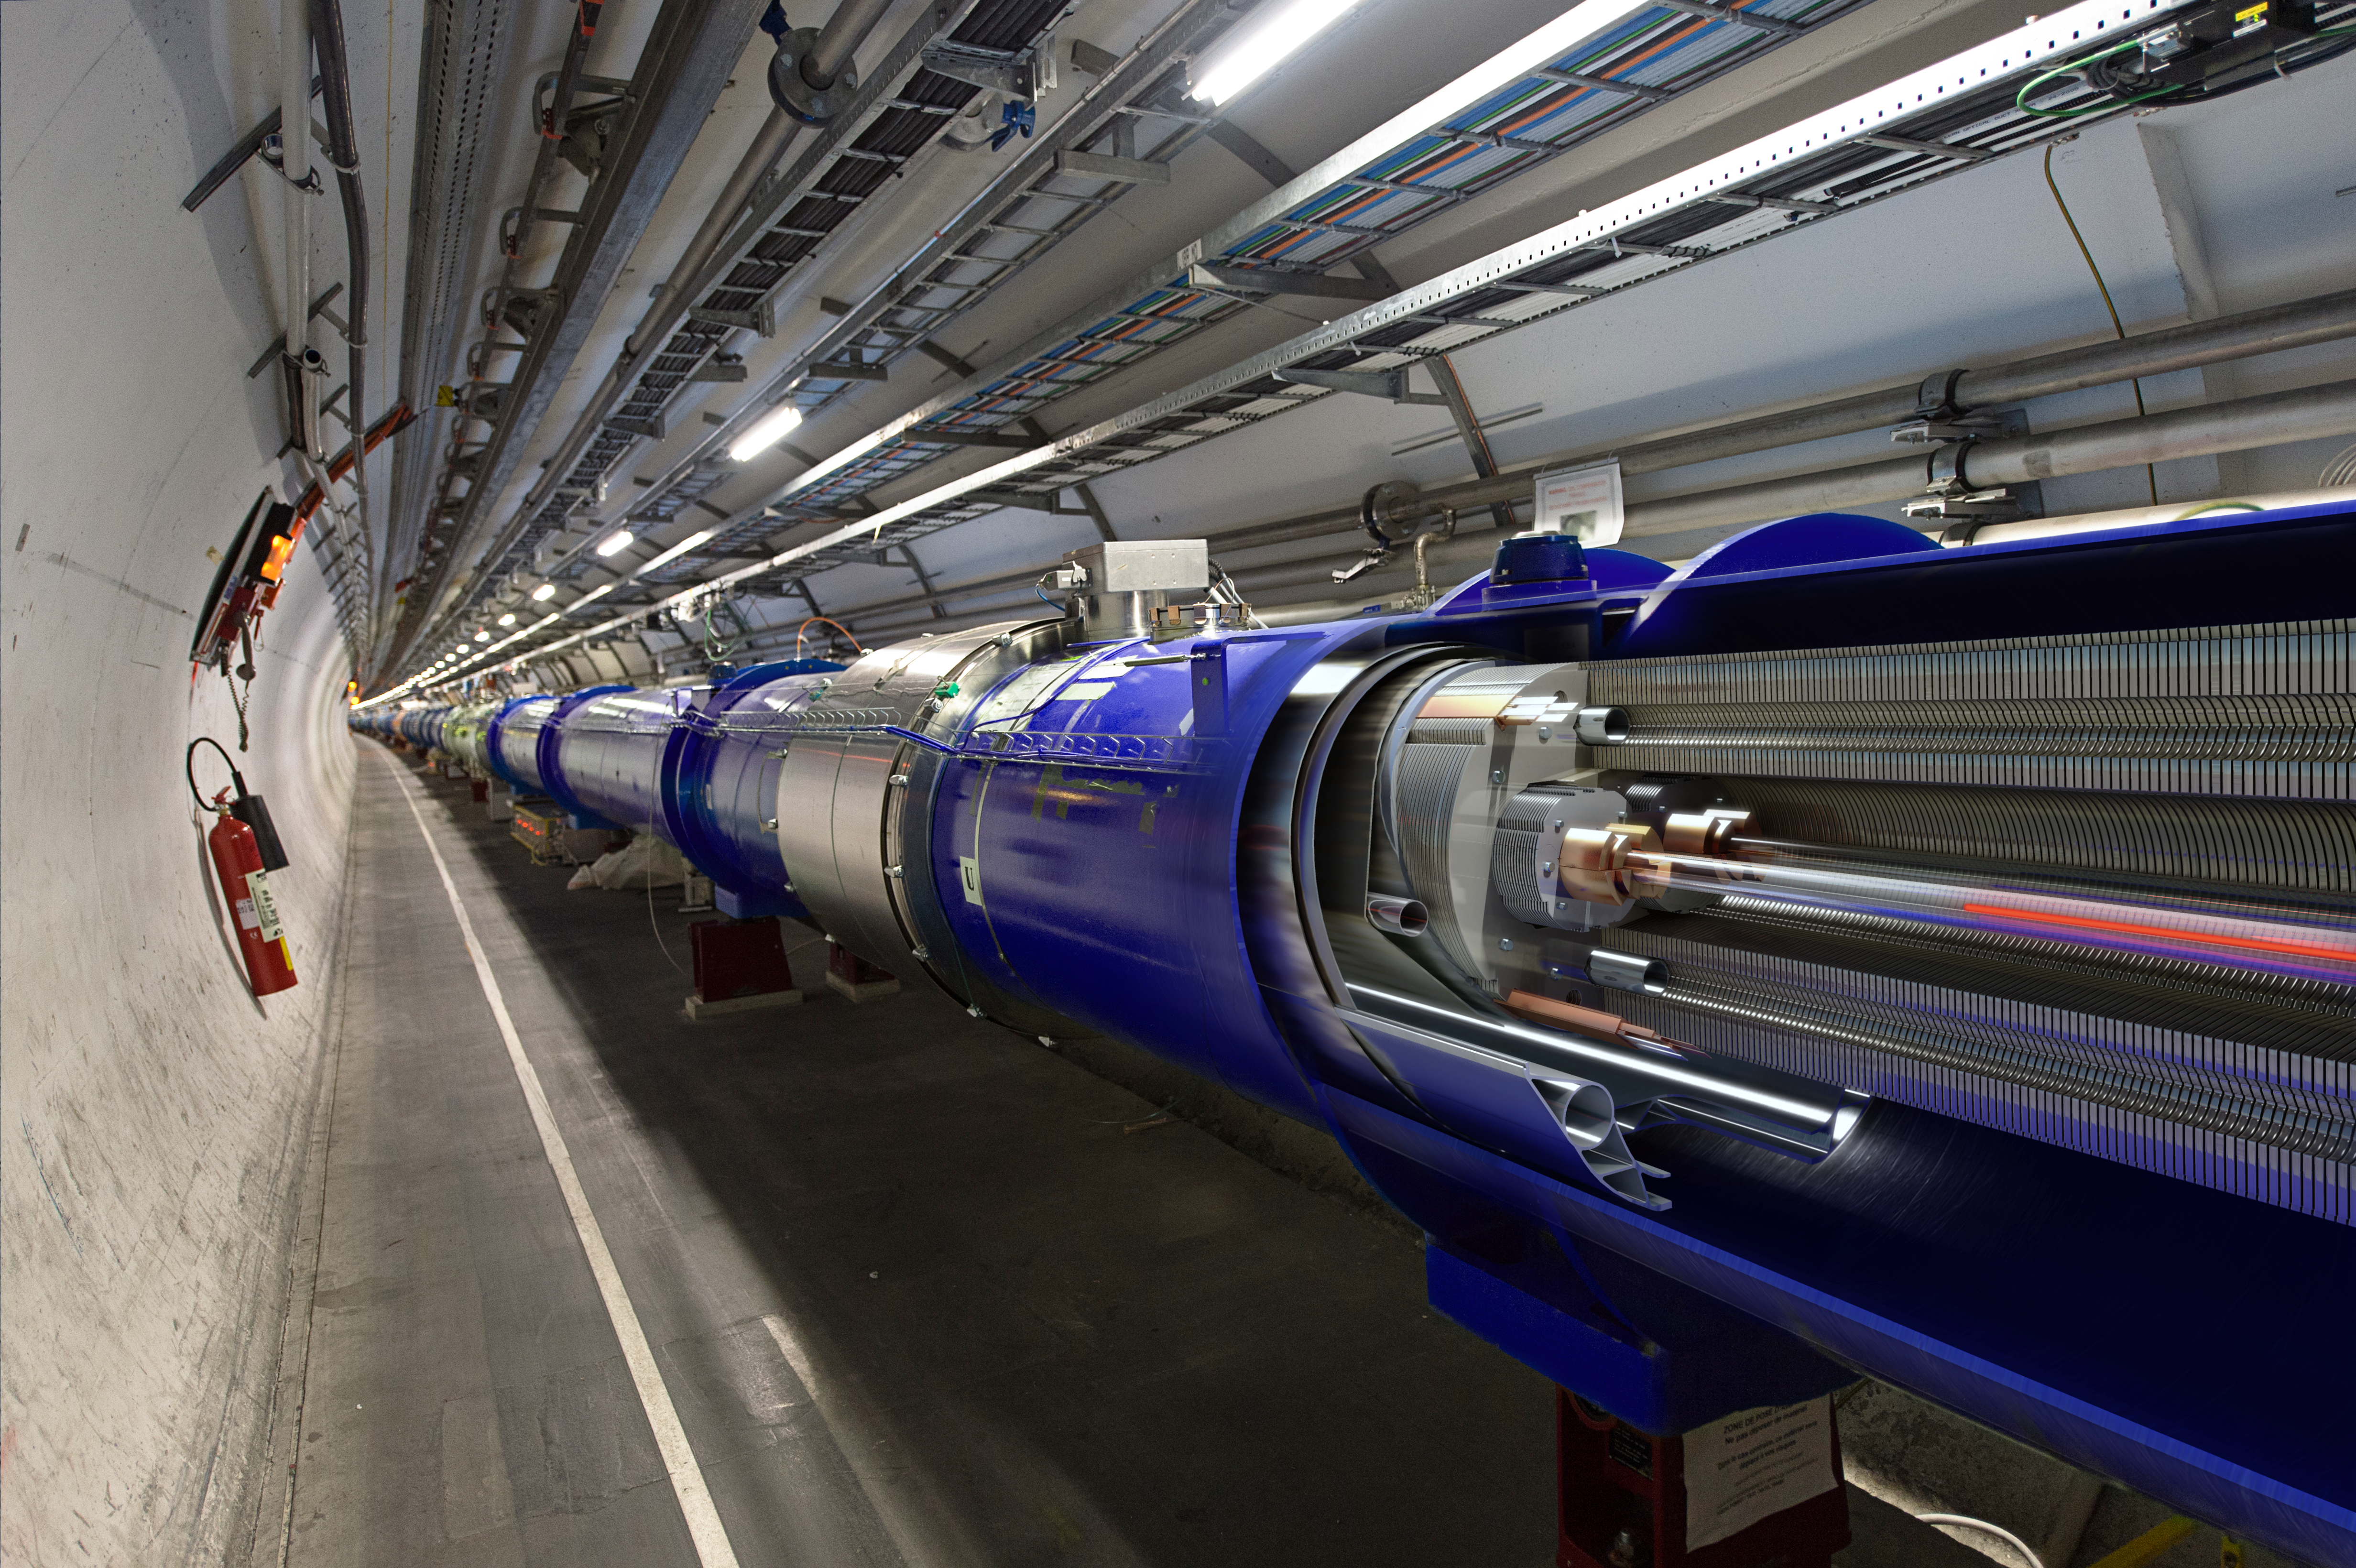
\includegraphics[width=0.8\textwidth]{chapters/01_Introduction/images/lhc_3D_cut.png}
    \caption{3D cut of a main LHC dipole~\cite{noauthor_cern_nodate}. Both beam pipes can be seen
    surrounded by the coils, strongly clamped by the yokes.}
    \label{fig:3d_cut_dipole}
\end{figure}


% -------------------------------
%   Straight Sections and Arcs
\subsubsection{\mread{Straight Sections and Arcs}}

The LHC is not a perfect circle. It is indeed composed of eight \textit{straight} sections, called
the \textit{Insertion Regions} (IRs) where detectors or specific instrumentation are placed.
Connecting those sections, the \textit{arcs} are where the majority of the magnets and their
correctors are located, along with some instrumentation like beam position monitors.
\Cref{fig:introduction:lhc_irs} shows the arcs as well as the purpose of each straight section.

\begin{figure}[!htb]
    \centering
    \includegraphics[width=0.5\textwidth]{./images/irs.png}
    \caption{Schematic of the LHC layout.}
    \label{fig:introduction:lhc_irs}
\end{figure}


% -------------------------------
%          Arc Cells
\subsubsection{\mread{Arc Cells}}

Each arc is made up of 23 cells. Magnets are organized in a standard FODO structure
(see \cref{section:courant_snyder}), as shown in \cref{fig:introduction:lhc_arc_cell}.
\textit{Dipoles} are responsible for bending the trajectory of the particles. Their associated
correctors, the orbit correctors, mitigate any possible drift in the path.
\textit{Quadrupoles} are used to control the beam size along the ring. Their effect is focusing in
one plane and defocusing in the other. Their associated correctors control the frequency of
oscillations of the beam (see tune, \cref{section:courant_snyder}) and possible field imperfections.
\textit{Sextupoles} correct chromaticity, a misfocus from quadrupoles due to particles having
a different momentum than the reference particle.
\textit{Octupoles} are used to stabilize the beam by introducing Landau
Damping~\cite{gareyte_landau_1997}. The associated correctors correct higher-order chromaticity
effects as well as amplitude-dependant tune shifts.
\textit{Decapoles} correctors aim at correcting an even higher chromaticity order.

\begin{figure}[H]
    \centering
    \includegraphics[width=1\textwidth]{./images/lhc_cell.png}
    \caption{Schematic of an LHC Arc cell~\cite{bruning_lhc_2004}.}
    \label{fig:introduction:lhc_arc_cell}
\end{figure}



% -------------------------------
%            Cycles
\subsubsection{\mread{Cycles}}

During the operation of the LHC, the machine goes through several states, each defined for specific 
scenarios~\cite{wenniger_lhc_2019}.

A common example is the operational cycle of the LHC, illustrated in \cref{fig:cern_complex:cycle}.
Initially, the magnets are pre-cycled~\cite{bottura_pre-cycles_2010} without any beam circulating,
to ensure a reproducible magnetic state. Their current is then increased to accept particles at the
injection energy of 450 GeV. To verify the machine's proper functioning, a probe bunch of reduced
intensity is first injected, at around $10^{10}$ particles. The number of bunches and their
intensity are then gradually increased to obtain the desired scheme needed for collisions, which
varies throughout the year based on experimental demands. The number of bunches and their intensity
can be adjusted as needed to ensure the machine's safety. A common scheme in 2024 is to inject about
2350 bunches, with around $1.5 \cdot 10^{11}$ particles in each bunch, for collisions. Optics
measurements, due to their destructive nature, typically use between one and three \textit{pilot}
bunches at a lower intensity of $10^{10}$ particles.

The current in the magnets is then increased along with adjustments in the phase and voltage of the
RF system to accelerate the particles to an energy of 6.8 TeV. During this ramp, the beam is
initially squeezed at the Interaction Points. However, further squeezing is limited by the
detectors' resolution, which is insufficient to accurately reconstruct a large number of collision
events simultaneously. Collisions then start, while levelling the $\beta^*$ at the ATLAS and CMS
experiments relative to the remaining beam intensity, ensuring optimal performance of the detectors.

\begin{figure}[!htb]
    \includegraphics[width=\textwidth]{./images/lhc_cycle.pdf}
    \caption{Simplified illustration of a standard LHC cycle. Adapted
    from~\cite{felix_soubelet_local_2023}.}
    \label{fig:cern_complex:cycle}
\end{figure}

% === Concepts of Accelerator Physics
\chapter{Concepts of Accelerator Physics}
\thumbforchapter{}
\chaptertoc{}
\newpage

\begin{enumerate}
    \tightlist
    \color{red}
    \item Hamiltonian
    \item Coordinates
    \begin{enumerate}
    \tightlist
        \item Courant Snyder, twiss parameters an phase space
        \item Linear Maps
        \item Non-Linear maps
        \item Normal Form \& RDT \& resonance diagram
    \end{enumerate}
    \item Linear optics: dispersion, coupling, momentum compaction
    \item Chromaticity

    \begin{enumerate}
    \tightlist
        \item Combined effect of multipoles
        \item Amplitude Detuning
        \item Chromtic Amplitude Detuning
        \item Dynamic Aperture
    \end{enumerate}
    \item Luminosity
\end{enumerate}



\input{chapters/02_Background/introduction.tex}
\section{Magnetic Fields}

% ============================================
%                Nomenclature
% ============================================
\subsection{\review{Nomenclature}}

Several notations coexist to denote magnetic fields. In this thesis, the
\textit{European Convention}~\cite{dilly_corrections_2022} is used for field indices, as shown
in Tab.~\ref{tab:magnetic_fields:relation_indices}. MAD-X, and MAD-NG, however, use the
\textit{American Convention}.

\begin{table}[H]
    \centering
    \begin{tabular}{l|c|c|c}
        Multipole     &      MAD-X        &     Index        & Normalized Strength \\
    \hline            
        Dipole        &     0             &     1            & $K_1$   \\       
        Quadrupole    &     1             &     2            & $K_2 $  \\
        Sextupole     &     2             &     3            & $K_3 $  \\
        Octupole      &     3             &     4            & $K_4 $  \\
        Decapole      &     4             &     5            & $K_5 $  \\
        Dodecapole    &     5             &     6            & $K_6 $  \\
        Decatetrapole &     6             &     7            & $K_7 $  \\
    \end{tabular}
    \caption{Relation between field indices and multipoles.}
    \label{tab:magnetic_fields:relation_indices}
\end{table}

As such, unless explicitly stated, quantities such as the magnetic strength $b$ and normalized
strength $K$ will be expressed with this notation. 


% ============================================
%              Multipole Expansion
% ============================================
\subsection{\review{Multipole Expansion}}

A 2 dimension magnetic field in the planes \textit{x} and \textit{y} can be described as a sum of
the normal and skew field gradients $\mathcal{B}$ and $\mathcal{A}$ with multipoles of order $n$,
given by~\cite{wolf_engineering_2001}:
\begin{equation}
    B_y + iB_x = \sum_{n=1}^\infty \left(\mathcal{B}_n + i\mathcal{A}_n \right)  (x+iy)^{n-1}
\end{equation}

An ideal magnet would produce either a sole normal or skew field. However, this is not applicable 
to real-life magnets that are imperfect, due to design and manufacturing constraints.
Field errors are thus introduced, relative to the main field of the ideal 2N-pole magnet at a
reference radius $r_{ref}$~\cite{dilly_corrections_2022}, as shown in 
Eq.~\eqref{eq:magnetic_field:relative_errors}. The coefficients of the normal and skew relative 
field errors, referred to as $a_n$ and $b_n$, are dimensionless but often given in \textit{units}
of $10^{-4}$.

\begin{equation}
    B_y + iB_x = 
        \begin{cases}
            \mathcal{B}_N \cdot \sum_{n+1}^\infty (b_n + ia_n) \left(\frac{x+iy}{r_{ref}}\right)^{n-1}\text{, for normal magnets}\\
            \mathcal{A}_N \cdot \sum_{n+1}^\infty (b_n + ia_n) \left(\frac{x+iy}{r_{ref}}\right)^{n-1}\text{, for skew magnets}
        \end{cases}
    \label{eq:magnetic_field:relative_errors}
\end{equation}


The normal and skew field components of order $n$ for an imperfect 2N-pole magnet is thus given by
the following equation:

\begin{equation}
    \begin{aligned}
        \mathcal{B}_n &= \mathcal{B}_N \cdot \frac{b_n}{r_{ref}^{n-1}}, \\
        \mathcal{A}_n &= \mathcal{A}_N \cdot \frac{a_n}{r_{ref}^{n-1}}.
    \end{aligned}
\end{equation}

The unit of the field is relative to the multipole order $n$: $[\text{Tm}^{1-n}]$.


% ============================================
%              Normalization
% ============================================
\subsection{\review{Beam Rigidity and Normalization}}

\subsubsection{\review{Beam Rigidity}}

The beam rigidity refers to the resistance of a particle moving through the accelerator to the
bending applied by the magnetic fields. It is derived from the Laurentz force~\cite{dilly_corrections_2022}
and relates the magnetic field $B$, the radius of curvature $\rho$ to the momentum $p$ and charge $q$
of the particle:

\begin{equation}
    B \rho = \frac{p}{q}
    \label{eq:magnetic_fields_beam_rigidity}
\end{equation}

It is of interest when designing an accelerator to set the maximum field as well as the required
radius of curvature for a specific momentum and particle.
An interesting metric of an accelerator is also its \textit{filling factor}, or percentage of
dipoles in the machine. It can be calculated via the radius of curvature: $f = \rho / r$. A low 
filling factors means more space for other magnets, collimators, beam instrumentation, etc.

\subsubsection{\review{Field Normalization}}

The Beam Rigidity is also used as a way to normalize magnetic field strengths in particle
accelerators where the momentum of the particle changes (i.e. acceleration).
Normalized Normal and Skew components $K_n$ and $J_n$ are given by~\cite{wolf_engineering_2001}:

\begin{equation}
    \begin{aligned}
        K_n =  \frac{q}{p} &(n-1)! \mathcal{B}_n, \\ 
        J_n =  \frac{q}{p} &(n-1)! \mathcal{A}_n.
    \end{aligned}
    \label{eq:magnetic_fields_normalized}
\end{equation}



% ============================================
%            Hamiltonian Dynamics
% ============================================
\subsection{Hamiltonian Dynamics}

\todo{link to lie algebra\\
poisson bracket is a link between hamiltonian and coordinate evolutions \\
Lie Algebra uses poisson brackets}

The Hamiltonian describing the motion for the transverse planes of a given multipole or order $n$ is
given by~\cite{keintzel_jacqueline_beam_nodate,tomas_direct_2003,franchi_studies_2006}:

\begin{equation}
    \begin{aligned}
        H &= \frac{q}{p} \Re \left[ \sum_{n>1} (\mathcal{B}_n + i\mathcal{A}_n) \frac{(x+iy)^n}{n} \right] \\
          &= \Re \left[ \sum_{n>1} (K_n + iJ_n) \frac{(x+iy)^n}{n!} \right].
    \end{aligned}
    \label{eq:hamiltonian_magnet}
\end{equation}

Quite often, when studying the effect of a magnet on the beam, only one component is required, and
the sum can thus be dropped.
The normal and skew fields can also be isolated in order to consider their effect only:

\begin{equation}
    \begin{aligned}
        N_n &= \frac{1}{n!} K_n \Re \left[ (x+iy)^n \right] \\
        S_n &= -\frac{1}{n!} J_n \Im \left[ (x+iy)^n \right].
    \end{aligned}
    \label{eq:normal_skew_hamiltonian_magnet}
\end{equation}




\section{Coordinate Systems}

In circular accelerators, particle dynamics are represented using a traveling coordinate system.
A reference orbit is determined by the lattice and its magnet strengths, forming the
\textit{optics}. In the case of a synchrotron, like the LHC, where the particles return to their
original location after some turns, the reference orbit is also called the closed orbit.  
The Frenet-Serret coordinate system is used, moving along the ring on the reference orbit. The
coordinates are then transverse: $x$ and $y$, and longitudinal in the direction of travel: $s$.
Figure~\ref{fig:coordinate_systems:frenet_serret} shows those coordinates.

\begin{figure}[H]
    \centering
    \includegraphics[width=0.6\textwidth]{example-image-a}
    \caption{\todo{Frenet-Serret coordinates commonly used in accelerator physics.}}
    \label{fig:coordinate_systems:frenet_serret}
\end{figure}



% ============================================
%               Linear Lattice 
% ============================================
\subsection{Linear Lattice}

A circular accelerator is composed of many multipoles of different orders. A basic
design only requires dipoles and quadrupoles in order to operate. Dipoles are used to bend the
particles in order to form the ring, whereas quadrupoles are used to focus the beam to a focal
point, similar to light optics.
Those elements can be arranged in a particular order, to form a \text{FODO} cell. Such cells present
an alternating placement of focusing an defocusing quadrupoles with dipoles in between, as shown in
Fig.\ref{fig:coordinate_systems:fodo}, and are usually repeated many times along the ring.

\begin{figure}[H]
    \centering
    \includegraphics[width=0.6\textwidth]{example-image-a}
    \caption{\todo{FODO cell, a repeated basic block present in most circular accelerators.}}
    \label{fig:coordinate_systems:fodo}
\end{figure}

A lattice composed on of only dipoles and quadrupoles, is referred to as a \textit{linear} lattice.

\todo{
    Courant Snyder/Twiss
    Tune, beta function
% 
    Lie, normal form
    Resonance Driving Terms
}
\section{Resonances}


%----------------------------------------
%
%----------------------------------------

\begin{figure}[H]
    \centering
    \includegraphics[width=0.7\textwidth]{images/resonance_diagaram_n5.png}
    \caption{Tune diagram with resonances lines excited by multipoles up to decapole ($n \leq 5$).
             The working point of the machine is chosen in an area where few lines are present.}
    \label{fig:resonances:diagram_n5}
\end{figure}


\begin{figure}[H]
    \centering
    \includegraphics[width=0.7\textwidth]{images/resonance_diagaram_n7.png}
    \caption{Tune diagram with resonances lines excited by multipoles up to decatetrapole 
             ($n \leq 7$). When considering higher orders, it becomes apparent that the beam will
             hit several resonances.}
    \label{fig:resonances:diagram_n7}
\end{figure}
\section{Detuning Effects}


% ============================================
%                Chromaticity
% ============================================
\subsection{\review{Chromaticity}}

Chromaticity is the tune change $\Delta Q$ relative to the momentum offset $\delta$. Chromaticity
can be described by a Taylor expansion, given by

\begin{equation} 
    Q (\delta) = Q_0 + Q' \delta + \frac{1}{2!} Q'' \delta^2 + \frac{1}{3!} Q''' \delta^3 + \mathcal{O}(\delta^4).
    \label{eq:background_chromaticity}
\end{equation}

Or, more generally, rewritten as a sum to include all orders up to $n$:

\begin{equation}
    Q (\delta) = Q_0 + \sum_{i=1}^n \frac{1}{i!} Q^{(i)} \delta^i.
    \label{eq:background_chromaticity_sum}
\end{equation}


The first order of the chromaticity expansion, $Q'$, is generally simply referred to as 
\textit{chromaticity}, sometimes as \textit{linear chromaticity}.
The other terms are thus referred to as \textit{non-linear chromaticity}.

The chromaticity change induced by a single element of order $n$ and length $L$ can be derived from
the Hamiltonian of Eq.~\eqref{eq:hamiltonian_magnet}, averaging over the phase variables and
differentiating relative to the actions $J_{x,y}$ and the momentum offset $\delta$:

\begin{equation}
    \Delta Q^{(n)}_{x,y} = \frac{\partial^n Q_{x,y}}{\partial^n \delta} = 
      \frac{1}{2\pi} \int_L \left< \frac{\partial^{(n+1)} H}{\partial J_{x,y}\partial^n \delta}\right> \diff s.
    \label{eq:background_chroma_order_hamiltonian}
\end{equation}


% =========
\subsubsection{Natural Chromaticity from Quadrupoles}

In a purely linear lattice, the linear chromaticity, $Q'$, is a result of the momentum dependence 
of the quadrupoles' focusing. It is in this case called the \textit{natural chromaticity} and can be
derived from the normal hamiltonian of Eq.\eqref{eq:normal_skew_hamiltonian_magnet} and expressing
the normalized magnet strength $K$ with a dependence on $\delta$ via $P$ as $P_0(1+\delta)$:

\begin{equation}
    K_n = \frac{q}{P_0} \frac{1}{1 + \delta} (n - 1)! B_n
    \label{eq:k_dpp}
\end{equation}

The normal field of a quadrupole is then given by

\begin{equation}
    \mathcal{N}_2(x,y) = \frac{1}{2} \frac{q}{P_0} \frac{1}{1+\delta} B_2 (x^2 - y^2)
\end{equation}

By operating a variable change to the angle coordinates 
(\(x \rightarrow \sqrt{2 J_x \beta_x} \cos \phi_x\) and
\(y \rightarrow \sqrt{2 J_y \beta_y} \cos \phi_y\)), the following equation linking the $\beta$-function
and $\delta$ to the normal field is obtained:
\begin{equation}\mathcal{N}_2 (x,y) = \frac{1}{2} \frac{q}{P_0} \frac{1}{1+\delta} B_2 
        \left[
            \left(\sqrt{2 J_x \beta_x} \cos \phi_x \right)^2 
            - \left(\sqrt{2 J_y \beta_y} \cos \phi_y\right)^2
        \right].
    \label{eq:hamiltonian_quadrupole_angle}
\end{equation}

Following Eq.\eqref{eq:background_chroma_order_hamiltonian}, the natural chromaticity $Q'$ induced by
quadrupoles is given by:
\begin{equation}
    \begin{aligned}
        \Delta Q'_x &= \frac{1}{2\pi} \int_L \frac{\partial^2 \left< \mathcal{N}_2 \right> }{\partial J_x \partial \delta} \diff s
        \quad;\quad
        \Delta Q'_y &= \frac{1}{2\pi} \int_L \frac{\partial^2 \left< \mathcal{N}_2 \right>}{\partial J_y \partial \delta} \diff s
        \\
        & = - \frac{1}{4 \pi} \frac{q}{P_0} B_2 L \beta_x
        & = \frac{1}{4 \pi} \frac{q}{P_0} B_2 L \beta_y
    \end{aligned}
\end{equation}


% =========
\subsubsection{Linear Chromaticity from Sextupoles}

The first order chromaticity $Q'$ is contributed to by sextupoles in the presence of off-momentum
particles. The normal field of a sextupole, following Eq.\eqref{eq:normal_skew_hamiltonian_magnet}
is given by

\begin{equation}
    \mathcal{N}_3(x,y) = \frac{1}{3!} (x^3 - 3xy^2).
    \label{eq:detuning:linear_chromaticity}
\end{equation}

As the momentum offset $\delta$ introduces a change in orbit via
dispersion~\cite{keintzel_second-order_2019}, a variable change can be operated on both $x$ and $y$,
as shown in Eq.\eqref{eq:detuning:offset}. In this thesis, vertical dispersion will be though
neglected.

\begin{equation}
    \begin{aligned}
        x &\rightarrow x + \Delta x = x + D_x\delta \\
        y &\rightarrow y + \Delta y = y + D_y\delta
    \end{aligned}
    \label{eq:detuning:offset}
\end{equation}

The positions $x$ and $y$ can once be replaced, using the twiss parameters, giving the full
expression:

\begin{equation}\begin{aligned}
  \mathcal{N}_3(x + \Delta x, y) = \frac{1}{6} K_3 \biggl[&
       \left(\sqrt{2 J_x \beta_x} \cos \phi_x\right)^3 \\
  &    + 3 \left(\sqrt{2 J_x \beta_x} \cos \phi_x\right)^2 D_x \delta \\
  &    + 3 \left(\sqrt{2 J_x \beta_x} \cos \phi_x\right) D_x^2 \delta^2 \\
  &    + D_x^3 \delta^3 \\
  &    - 3 \left(\sqrt{2 J_x \beta_x} \cos \phi_x \right) \left(\sqrt{2 J_y \beta_y} \cos \phi_y \right)^2 \\
  &    - 3 D_x \delta (\sqrt{2 J_y \beta_y} \cos \phi_y)^2 \biggl]
\end{aligned}\end{equation}

Averaging over the phase variables removes any odd cosine:
\begin{equation}\begin{aligned}
  \left< \mathcal{N}_3(x + \Delta x, y) \right> = \frac{1}{6} K_3 &\biggl(
       3 J_x \beta_x D_x \delta \\
  &    + D_x^3 \delta^3 \\
  &    - 3 D_x \delta J_y \beta_y \biggl)
\end{aligned}\end{equation}



The chromaticity can then obtained by differentiating relative to the action $J_{x,y}$ to obtain the
tune, and then by the momentum offset $\delta$.
\begin{equation}
    \begin{aligned}
        \Delta Q'_x &= \frac{1}{2\pi} \int_L \frac{\partial^2 \left< \mathcal{N}_3 \right>}{\partial J_x \partial \delta} \diff s \quad; \quad \Delta Q'_y &&= \frac{1}{2\pi} \int_L \frac{\partial^2 \left< \mathcal{N}_3 \right>}{\partial J_y \partial \delta} \diff s \\
        &= \frac{1}{2 \pi} L \frac{1}{2} K_3 \beta_x D_x  &&= - \frac{1}{2 \pi} L \frac{1}{2} K_3 \beta_y D_x \\
        &= \frac{1}{4 \pi}  K_3 L \beta_x D_x &&= - \frac{1}{4 \pi}  K_3 L \beta_y D_x
    \end{aligned}
\end{equation}

From this last equation, it is apparent than sextupoles are not a source of chromaticity of higher
orders in the presence of linear dispersion. In the presence of second order
dispersion~\cite{keintzel_second-order_2019}, sextupoles can generate some amount of $Q''$, usually
negligible.


% =========
\subsubsection{Non-Linear Chromaticity}

Higher orders of the chromaticity function are described in~\cite{dilly_derivation_2023} and follow
the same logic as for the linear chromaticity from sextupoles.





% ============================================
%             Amplitude Detuning
% ============================================
\subsection{Amplitude Detuning}



% ============================================
%        Chromatic Amplitude Detuning
% ============================================
\subsection{Chromatic Amplitude Detuning}

\todo{make it clear I derived it}
\chapter{Optics Measurements and Corrections}

% === Beam Instrumentation
\section{Beam Instrumentation}

% === Measurements
\section{Optics Measurements}

% tbt
% chromaticity

\section{Correction Concepts}
\chapter{Theory}
\thumbforchapter{}
\chaptertoc{}

\section{Units}\label{units}

\begin{itemize}
\item
  Joules: \[1 J = 1 N \cdot m = 1 kg \cdot m^2 \cdot s^{-2}\]
\item
  Electronvolt:

  \begin{itemize}
  \tightlist
  \item
    \(eV = e \cdot V\)

    \begin{itemize}
    \tightlist
    \item
      e: elementary charge
    \item
      V: volt
    \end{itemize}
  \item
    \(1 eV = 1.602176634 \cdot 10^{-19} J\)
  \end{itemize}
\item
  Momentum:

  \begin{itemize}
  \tightlist
  \item
    \(p\) in \(kg.m.s^{-1}\)
  \item
    \(p\) in \(eV.c^{-1}\): \(J \cdot c^{-1} = kg.m.s^{-1}\)
  \end{itemize}
\item
  Tesla \[T = \frac{V \cdot s}{m}\]
\end{itemize}

\newpage

\hypertarget{definitions}{%
\section{Definitions}\label{definitions}}

\hypertarget{some-math-definitions}{%
\subsection{Some Math Definitions}\label{some-math-definitions}}

\begin{itemize}
\item
  Harmonic Oscillator \[F = -kx\] \[x'' = -\frac{k}{m}x \]
\item
  Magnetic rigidity, used for dipoles: \[B\rho = \frac{p}{q}\]

  \begin{itemize}
  \item
    B: magnetic field {[}\(T\){]}
  \item
    \(\rho\): radius of curvature of the orbit {[}\(m\){]}
  \item
    p: momentum {[}\(eV/c\){]}
  \item
    q: particle charge {[}\(e\){]}
  \item
    Can be expressed as \[B \rho = 3.3356 p\] if \(p\) is in GeV/c
  \end{itemize}
\item
  Magnets orders
\end{itemize}

\begin{center}
  \begin{tabular}{lllllll}
  Magnet Letter          & B & Q & S & O & D & T \\
  Number of Poles        & 2 & 4 & 6 & 8 & 10 & 12 \\
  a (skew) designation   & 1 & 2 & 3 & 4 & 5 & 6 \\
  b (normal) designation & 1 & 2 & 3 & 4 & 5 & 6 \\
  K designation          & 1 & 2 & 3 & 4 & 5 & 6 \\
  MADX-K                 & 0 & 1 & 2 & 3 & 4 & 5 \\
  \end{tabular}
\end{center}

\begin{itemize}
\item
  Magnet Strength:
  \begin{equation}K_{n} = \frac{q}{P} (n-1)!B_n\label{eq:magnet_strength}\end{equation}

  \begin{itemize}
  \item
    The unit is given by:

    \begin{itemize}
    \tightlist
    \item
      k1: dipole: \(m^{-1}\)
    \item
      k2: quadrupole: \(m^{-2}\)
    \item
      k3: sextupole: \(m^{-3}\)
    \item
      k4: octupole: \(m^{-4}\)
    \item
      k5: decapole: \(m^{-5}\)
    \item
      k6: dodecapole: \(m^{-6}\)
    \end{itemize}
  \item
    If interested in the \emph{integrated} strength, multiply by
    \emph{m}
  \end{itemize}
\item
  Dispersion is given via:
  \begin{equation}D = \frac{\Delta x}{\delta}\end{equation}
\item
  The relative momentum offset is defined via the reference momentum and
  the momentum
  \begin{equation}\delta = \frac{\Delta P}{P_0} = \frac{P - P_0}{P_0}\label{eq:dpp}\end{equation}
\item
  Relation between the action and the single particle emittance:
  \href{https://journals.aps.org/prab/pdf/10.1103/PhysRevSTAB.17.081002}{Non
  Linear Observables} (eq. 2):
  \begin{equation}2J_{x,y} = \epsilon_{x,y}\end{equation}
\item
  The tune is defined as the derivative of the Hamiltonian relative to
  the action.
  \begin{equation}Q_{x,y} = \frac{\partial \left< H \right>}{\partial J_{x,y}}\end{equation}
\item
  The tune can also be defined as:
  \begin{equation}Q_{x,y} = \frac{1}{2 \pi} \oint \frac{1}{\beta_{x,y}(s)} \,ds\end{equation}
\item
  The phase advance in the \(x\) plane, between two elements \(w\) and
  \(j\), in the accelerator is given by
  \href{https://arxiv.org/abs/1711.06589}{AnalyticFormulasFranchi}:
\end{itemize}

\begin{equation}
\begin{cases} 
  \Delta \phi_{x,wj} = \left(\phi_{x,j} - \phi_{x,w} \right)              & \mbox{if } \phi_{x,j} > \phi_{x,w}, \\
  \Delta \phi_{x,wj} = \left(\phi_{x,j} - \phi_{x,w} \right) + 2 \pi Q_x  & \mbox{if } \phi_{x,j} < \phi_{x,w}.
\end{cases}
\end{equation}

\newpage

\hypertarget{maths}{%
\section{Maths}\label{maths}}

\hypertarget{taylor-series}{%
\subsection{Taylor Series}\label{taylor-series}}

The Taylor series of a multivariable function at the point
\((a_1, \cdots, a_d)\) is defined as:

\begin{equation}\begin{aligned}
  f(x_1, \cdots, x_d) = &f(a_1, \cdots, a_d) \\
                &+ \frac{1}{1!} \sum_{j=1}^{d} \frac{\partial f(a_1, \cdots, a_d)}{\partial x_j} (x_j - a_j) \\
                &+ \frac{1}{2!}\sum_{j=1}^{d}\sum_{k=1}^{d} \frac{\partial^2 f(a_1, \cdots, a_d)}{\partial x_j\partial x_k} (x_j - a_j) (x_k - a_k) \\
                &+ \frac{1}{3!}\sum_{j=1}^{d}\sum_{k=1}^{d}\sum_{l=1}^{d} \frac{\partial^3 f(a_1, \cdots, a_d)}{\partial x_j\partial x_k\partial x_l} (x_j - a_j) (x_k - a_k) (x_l - a_l)\\
                &+ \cdots
\end{aligned}\label{eq:taylor}\end{equation}

\hypertarget{non-linear-transfer-maps}{%
\subsection{Non-Linear Transfer Maps}\label{non-linear-transfer-maps}}

For linear dynamics, linear transfer maps can be used to describe a
particle's position from the elements in the lattice and the particle's
current position. In the non linear case, such a formalism can't be
used. Instead, the Lie operator is used.

\hypertarget{lie-operator}{%
\subsubsection{Lie Operator}\label{lie-operator}}

Resources found in
\href{https://mlegarre.web.cern.ch/mlegarre/Courses/Meghan_RDTpresentation.pdf}{Meghan
McAteer's talk} and Wolski's book.

The Lie operator is defined as:

\[
\colon f \colon = \sum^n_{i=1} \left(\frac{\partial f}{\partial x_i} \frac{\partial}{\partial p_i} 
                           - \frac{\partial f}{\partial p_i} \frac{\partial}{\partial x_i}
                      \right)
\]

With \emph{i} the index of a dimension. So \(x_1\) would be \(x\) and
\(x_2\), \(y\).

The exponential Lie operator \(e^{:f:}\) acting on a function \(g\):

\begin{equation}e^{:f:}g = g + [f, g] + \frac{1}{2} [f, [f, g]] + \cdots\label{eq:Lie}\end{equation}

This is from the usual power series of an exponential:

\[e^{:f:} = \sum^{\infty}_{m=0} \frac{:f:^m}{m!}\]

Where \([f, g]\) is a poisson bracket, still somehow used for historical
reasons:

\begin{equation}[f, g] = \colon f \colon g
\label{eq:poisson_bracket}\end{equation}

Thus, the particle with coordinates \(\vec{x}\) passing through an
element can be mapped using the Hamiltonian of the element (Wolski, eq.
9.6):

\begin{equation}\vec{x}_f = e^{-\Delta s:H:} \vec{x}_0\label{eq:position_non_linear}\end{equation}

For a \emph{thin} lens, we can directly multiply by the length of the
magnet:

\begin{equation}\vec{x}_f = e^{-L:H:} \vec{x}_0\label{eq:position_non_linear_thin}\end{equation}

By combining \cref{eq:Lie} and \cref{eq:position_non_linear}, we obtain:

\begin{equation}
\begin{aligned}
\left[H, \vec{x}_0\right] =& \frac{\partial H}{\partial x} \frac{\partial \vec{x}_0}{\partial p_x} 
                                    -\frac{\partial H}{\partial p_x} \frac{\partial \vec{x}_0}{\partial x} \\
                           &\frac{\partial H}{\partial y} \frac{\partial \vec{x}_0}{\partial p_y} 
                                    -\frac{\partial H}{\partial p_y} \frac{\partial \vec{x}_0}{\partial y}
\end{aligned}
\label{eq:bracket_hamiltonian}\end{equation}

Thus giving us the complete equation:

\begin{equation}
\begin{aligned}
\vec{x}_f &= e^{:H:}\vec{x}_0 \\
          &= \vec{x}_0 + \left[H, \vec{x}_0\right] \\
          &= \begin{pmatrix} x \\ p_x \\ y \\ p_y\end{pmatrix}_0
             + \begin{pmatrix} -\frac{\partial H}{\partial p_x} \\ 
                               \frac{\partial H}{\partial x} \\
                               -\frac{\partial H}{\partial p_y} \\
                               \frac{\partial H}{\partial y}
               \end{pmatrix} \\
\begin{pmatrix} x \\ 
                p_{x} \\
                y \\
                p_{y} 
\end{pmatrix}_f
          &=  \begin{pmatrix} x_0 - \dfrac{\partial H}{\partial p_x} \\ 
                               p_{x0} +\dfrac{\partial H}{\partial x} \\
                               y_0 - \dfrac{\partial H}{\partial p_y} \\
                               p_{y0} +\dfrac{\partial H}{\partial y}
               \end{pmatrix}
\end{aligned}
\label{eq:non_linear_map}\end{equation}

This non linear transfer map is a general map without coupling.

\hypertarget{multipole-expansion}{%
\subsection{Multipole Expansion}\label{multipole-expansion}}

This is the Hamiltonian for a magnetic element with normal strength
component \emph{K} and skew component \emph{J}:

\begin{equation}H = \Re \left[\sum_{n>1} \left( K_{n} + iJ_{n} \right) \frac{(x+iy)^n}{n!} \right]\label{eq:hamiltonian}\end{equation}

This equation is an expansion of the magnetic field into its multipole
components. If we're only interested in one component, the sum can be
dropped and \(n\) set to the desired multipole.

Remark: When writing terms like \(K_1\) it is assumed it is \(K_1(s)\).
Is is important later for the chromaticity where the average is a
circular integral over s.

It follows that the normal and skew fields are:

\begin{equation}\mathcal{N}_n = \frac{1}{n!}K_n \Re \left[(x+iy)^n\right]\end{equation}
\begin{equation}\mathcal{I}_n = -\frac{1}{n!}J_n \Im \left[(x+iy)^n\right]\end{equation}

\hypertarget{quadrupole}{%
\subsubsection{Quadrupole}\label{quadrupole}}

\begin{equation}\mathcal{N_2}(x, y) = \frac{1}{2} K_2 (x^2 - y^2)\end{equation}

\hypertarget{sextupole}{%
\subsubsection{Sextupole}\label{sextupole}}

\begin{equation}\mathcal{N_3}(x, y) = \frac{1}{6} K_3 (x^3 - 3xy^2)\end{equation}

\hypertarget{octupole}{%
\subsubsection{Octupole}\label{octupole}}

\begin{equation}\mathcal{N_4}(x, y) = \frac{1}{24} K_4 (x^4 - 6x^2y^2 + y^4)\end{equation}

\hypertarget{decapole}{%
\subsubsection{Decapole}\label{decapole}}

\begin{equation}\mathcal{N_5}(x, y) = \frac{1}{120} K_5 (x^5 - 10x^3y^2 + 5xy^4)\end{equation}

\hypertarget{dodecapole}{%
\subsubsection{Dodecapole}\label{dodecapole}}

\begin{equation}\mathcal{N_6}(x, y) = \frac{1}{720} K_6 (x^6 - 15x^4y^2 + 15x^2y^4 - y^6)\end{equation}

\hypertarget{multinomial-expansion}{%
\subsection{Multinomial Expansion}\label{multinomial-expansion}}

For any positive integer \emph{m} and non-negative integer \emph{n}, the
multinomial expansion describes the expansion of a sum raised to the
power \emph{n}.

\begin{equation}
(x_1 + x_2 + \cdots + x_m)^n = \sum_{k_1 + k_2 + k_3 + \cdots + k_m = n} 
                               \frac{n!}{k_1!k_2!\cdots k_m!}
                               x_1^{k_1}x_2^{k_2}x_1^{k_2} \cdots x_m^{k_m}
\label{eq:multinomial_expansion}\end{equation}

It should be noted that the sum \(k_1 + k_2 + \cdots + k_m\) is
\emph{equal} to \(n\). This avoids unwanted terms in the expansion.
Another form of writing the multinomial expansion is with the Kronecker
delta, notice that here the sum is \emph{less than or equal} to \(n\):

\begin{equation}\delta_{i,j} = 
\begin{cases} 
  0 & \mbox{if } i \neq j, \\
  1 & \mbox{if } i = j.
\end{cases}
\label{eq:kronecker}\end{equation}

\begin{equation}
(x_1 + x_2 + \cdots + x_m)^n = \sum_{k_1 + k_2 + k_3 + \cdots + k_m \leq n} \delta_{j + k + l + m,n}
                               \frac{n!}{k_1!k_2!\cdots k_m!}
                               x_1^{k_1}x_2^{k_2}x_1^{k_2} \cdots x_m^{k_m}
\label{eq:multinomial_expansion_kronecker}\end{equation}

\hypertarget{example}{%
\subsubsection{Example}\label{example}}

\begin{equation}
\begin{aligned}
(a + b + c + d)^n &= \sum_{j + k + l + m = n} 
                      \frac{n!}{j!k!l!m!}
                      a^j b^k c^l d^m  \\
                  &= \sum_{j + k + l + m \leq n} 
                      \delta_{j + k + l + m,n}
                      \frac{n!}{j!k!l!m!}
                      a^j b^k c^l d^m  \\
                  &= \sum^n_{j=0}\sum^n_{k=0}\sum^n_{l=0}\sum^n_{m=0}
                      \delta_{j + k + l + m,n}
                      \frac{n!}{j!k!l!m!} 
                      a^j b^k c^l d^m
\end{aligned}
\end{equation}

This expansion is particularly useful for Resonance Driving Terms (RDTs)
to isolate specific resonances.

\newpage

\hypertarget{non-linear-transfer-maps-1}{%
\section{Non-Linear Transfer Maps}\label{non-linear-transfer-maps-1}}

This section details the transfer maps for each multipole. The used
transfer map is the non linear map defined by \cref{eq:non_linear_map}.

\hypertarget{quadrupole-1}{%
\subsection{Quadrupole}\label{quadrupole-1}}

The main normal field of a quadrupole is defined by:

\begin{equation}
\begin{aligned}
  H &= \frac{1}{2} K_2 (x^2 - y^2) \\
    &= \frac{1}{2} \frac{q}{P} B_2 (x^2 - y^2)
\end{aligned}
\end{equation}

We can now differentiate the Hamiltonian to find the needed terms:

\begin{equation}
\begin{aligned}
\frac{\partial H}{\partial x} &= \frac{q}{P_0} B_2 x &; \quad \frac{\partial H}{\partial y} &= -\frac{q}{P_0} B_2 y \\
\frac{\partial H}{\partial p_x} &= 0                 &; \quad \frac{\partial H}{\partial p_y} &= 0
\end{aligned}
\end{equation}

We then get the equation for a thin quadrupole we're familiar with.
Please note the addition of the term \(-L\) into the power series of the
exponential, which leads to reversed signs:

\begin{equation}\begin{aligned}
\begin{pmatrix}
x \\ p_x \\ y \\ p_y
\end{pmatrix}_f
& =
\begin{pmatrix}
x_0 \\
p_{x0} - \dfrac{q}{P_0} L B_2 x_0 \\
y_0 \\
p_{y0} + \dfrac{q}{P_0} L B_2 y_0 \\
\end{pmatrix}\\
& =
\begin{pmatrix}
x \\ p_x \\ y \\ p_y
\end{pmatrix}_0
-\frac{q}{P_0}LB_2
\begin{pmatrix}
0 \\ x_0 \\ 0 \\ y_0
\end{pmatrix}\\
& =
\begin{pmatrix}
1 & 0 & 0 & 0 \\ -\dfrac{q}{P_0}LB_2 & 1 & 0 & 0 \\ 0 & 0 & 1 & 0 \\ 0 & 0 & \dfrac{q}{P_0}LB_2 & 1
\end{pmatrix}
\begin{pmatrix}
x \\ p_x \\ y \\ p_y
\end{pmatrix}_0
\end{aligned}\end{equation}

\hypertarget{sextupole-1}{%
\subsection{Sextupole}\label{sextupole-1}}

The main normal field of a sextupole is defined by:

\begin{equation}
\begin{aligned}
  H &= \frac{1}{6} K_3 (x^3 - 3xy^2) \\
    &= \frac{1}{3} \frac{q}{p} B_3 (x^3 - 3 xy^2)
\end{aligned}
\end{equation}

We can now differentiate the Hamiltonian to find the needed terms:

\begin{equation}
\begin{aligned}
\frac{\partial H}{\partial x} &= \frac{q}{P_0} B_3 (x^2 - y^2) &; \quad \frac{\partial H}{\partial y} &= -2 \frac{q}{P_0} B_3 x y \\
\frac{\partial H}{\partial p_x} &= 0                 &; \quad \frac{\partial H}{\partial p_y} &= 0
\end{aligned}
\end{equation}

We then get:

\begin{equation}
\begin{pmatrix}
x \\ p_x \\ y \\ p_y
\end{pmatrix}_f
=
\begin{pmatrix}
x_0 \\
p_{x0} - \dfrac{q}{P_0} L B_3 (x_0^2 - y_0^2) \\
y_0 \\
p_{y0} + 2\dfrac{q}{P_0} L B_3 x_0 y_0 \\
\end{pmatrix}
\end{equation}

\newpage

\hypertarget{chromaticity}{%
\section{Chromaticity}\label{chromaticity}}

The chromaticity is the change of tune relative to the relative offset
momentum. It is thus given by Eq.(5.5) of
\href{https://cds.cern.ch/record/1951379/files/Thesis-2014-Ewen}{Ewen's
Thesis}:

\[Q'_{x,y} = \frac{\partial Q_{x,y}}{\partial \delta} = \frac{1}{2\pi}\left< \frac{\partial² H}{\partial J_{x,y}\partial \delta}\right>\]

For a single element, we can compute $\Delta Q'$:
\begin{equation}\Delta Q_{x,y}' = \frac{1}{2\pi} \int_L \frac{\partial^2 \left< H \right>}{\partial J_{x,y} \partial \delta} \diff s\label{eq:chroma}\end{equation}

By doing a Taylor Expansion on \(Q(\delta)\), we get:

\begin{equation} Q (\delta) = Q_0 + Q' \delta + \frac{1}{2!} Q'' \delta^2 + \frac{1}{3!} Q''' \delta^3 ... \label{eq:tune_chroma}\end{equation}

\newpage

\hypertarget{quadrupole-2}{%
\subsection{Quadrupole}\label{quadrupole-2}}

Full expression of the Hamiltonian for the magnet given by eq.
\ref{eq:hamiltonian} :
\begin{equation}H_2(x,y) = \frac{1}{2} K_2 (x^2 - y^2) - J_2 xy\label{eq:hamiltonian_quadrupole}\end{equation}

Magnets usually only have a main field and aren't skewed. We can keep
only the main normal field:
\begin{equation}\mathcal{N}_2(x,y) = \frac{1}{2} K_2 (x^2 - y^2)\label{eq:main_hamiltonian_quadrupole}\end{equation}

In a region of zero dispersion, we can write
\(x \rightarrow x + \Delta x \Longleftrightarrow x \rightarrow x + \eta \delta\)
with \(\eta\) being the dispersion and \(\delta\) the relative momentum
offset \(\delta p / p_0\). This bring us to:
\begin{equation}\mathcal{N}_2 (x,y) = \frac{1}{2} K_2 ((x + \eta \delta)^2 - y^2)\label{eq:hamiltonian_quadrupole_dpp}\end{equation}

By operating a variable change to the angle coordinates
(\(x = \sqrt{2 J_x \beta_x} \cos \phi_x\) and
\(y = \sqrt{2 J_y \beta_y} \cos \phi_y\)):
\begin{equation}\mathcal{N}_2 (x,y) = \frac{1}{2} K_2 \left[\left(\sqrt{2 J_x \beta_x} \cos \phi_x + \eta \delta\right)^2 - \left(\sqrt{2 J_y \beta_y} \cos \phi_y\right)^2\right]\label{eq:hamiltonian_quadrupole_angle}\end{equation}

We can then now differentiate relative the relative momentum offset
\(\delta\):
\begin{equation}\frac{\partial \mathcal{N_2}}{\partial \delta} =  \frac{1}{2} K_2 \left(\sqrt{2 J_x \beta_x} \cos \phi_x \eta + 2 \eta \delta\right)\label{eq:n2_dpp}\end{equation}

Differientiating relative to the action:
\begin{equation}\frac{\partial \mathcal{N_2}}{\partial J_x \partial \delta} =  \frac{1}{2} K_2 \left (\frac{2 \beta_x}{2 \sqrt{2 J_x \beta_x}} \cos \phi_x \eta \right) \end{equation}
\begin{equation}\frac{\partial \mathcal{N_2}}{\partial J_y \partial \delta} = 0\end{equation}

Averaging over the phase variables gives:
\begin{equation}\left< \frac{\partial \mathcal{N_2}}{\partial J_{x,y} \partial \delta} \right> = 0\end{equation}

From this approach, we can see we don't have any chromaticity induced by
quadrupoles. This is because we assumed the quadropole strength,
\(K_2\), was constant and not momentum dependant.

To find chromaticity from the \(K\) strength we need to change \(K\) and
express \(P\) as \(P_0(1 + \delta)\), combining eq.
\ref{eq:magnet_strength} and eq. \ref{eq:dpp}:
\begin{equation}K_n = \frac{q}{P_0} \frac{1}{1 + \delta} (n - 1)! B_n\label{eq:k_dpp}\end{equation}

Going back to eq. \ref{eq:hamiltonian_quadrupole_angle}, averaging it
and substituting \ref{eq:k_dpp}:
\begin{equation}\frac{\partial \left< \mathcal{N_2} \right>}{\partial J_x} = \frac{1}{2} \frac{q}{P_0} (1 - \delta) B_2 \beta_x\end{equation}
\begin{equation}\frac{\partial \left< \mathcal{N_2} \right>}{\partial J_y} = - \frac{1}{2} \frac{q}{P_0} (1 - \delta) B_2 \beta_y\end{equation}

Now that \(\delta\) is in the equation, we can differentiate by it:
\begin{equation}\frac{\partial^2 \left< \mathcal{N_2} \right>}{\partial J_x \partial \delta}  = - \frac{1}{2} \frac{q}{P_0} B_2 \beta_x\end{equation}
\begin{equation}\frac{\partial^2 \left< \mathcal{N_2} \right>}{\partial J_x \partial \delta}  = \frac{1}{2} \frac{q}{P_0} B_2 \beta_x\end{equation}

We can now get the chromaticity \(Q'\): \begin{equation}\begin{aligned}
\Delta Q'_x &= \frac{1}{2\pi} \int_L \frac{\partial^2 \left< \mathcal{N_2} \right> }{\partial J_x \partial \delta} \diff s \\
  & = - \frac{1}{4 \pi} \frac{q}{P_0} B_2 L \beta_x
\end{aligned}\end{equation}

\begin{equation}\begin{aligned}
\Delta Q'_y &= \frac{1}{2\pi} \int_L \frac{\partial^2 \left< \mathcal{N_2} \right>}{\partial J_y \partial \delta} \diff s \\
  & = \frac{1}{4 \pi} \frac{q}{P_0} B_2 L \beta_y
\end{aligned}\end{equation}

\newpage

\hypertarget{sextupole-2}{%
\subsection{Sextupole}\label{sextupole-2}}

Full expression of the Hamiltonian for the magnet given by eq.
\ref{eq:hamiltonian} :
\begin{equation}\mathcal{H_3}(x, y) = \frac{3 K_{2} \left(x^{2} - y^{2}\right)}{6} + \frac{K_{3} \left(x^{3} - 3 x y^{2}\right)}{6} - J_{2} x y - \frac{J_{3} \left(3 x^{2}y - y^{3}\right)}{6}\end{equation}

Main normal field:
\begin{equation}\mathcal{N_3}(x, y) = \frac{K_{3} \left(x^{3} - 3 xy^{2}\right)}{6}\end{equation}

With a displacement in x:
\begin{equation}\mathcal{N_3}(x + \Delta x, y) = \frac{K_{3} \left((x + \eta \delta)^{3} - 3 (x + \eta \delta)y^{2}\right)}{6}\end{equation}

Expanding:
\begin{equation}\mathcal{N_3}(x + \Delta x, y) = \frac{K_{3} \left(x^3 + 3 x^2 \eta \delta + 3 x \eta^2 \delta^2 + \eta^3 \delta^3 - 3xy^2 - 3 \eta \delta y^2 \right)}{6}\end{equation}

Changing variables:

\begin{equation}\begin{aligned}
  \mathcal{N_3}(x + \Delta x, y) = \frac{1}{6} K_3 \biggl[&
       \left(\sqrt{2 J_x \beta_x} \cos \phi_x\right)^3 \\
  &    + 3 \left(\sqrt{2 J_x \beta_x} \cos \phi_x\right)^2 \eta \delta \\
  &    + 3 \left(\sqrt{2 J_x \beta_x} \cos \phi_x\right) \eta^2 \delta^2 \\
  &    + \eta^3 \delta^3 \\
  &    - 3 \left(\sqrt{2 J_x \beta_x} \cos \phi_x \right) \left(\sqrt{2 J_y \beta_y} \cos \phi_y \right)^2 \\
  &    - 3 \eta \delta (\sqrt{2 J_y \beta_y} \cos \phi_y)^2 \biggl]
\end{aligned}\end{equation}

It is faster and easier here to average over the phase variables before
differentiating. Any odd cosine can be removed since its average is 0:
\begin{equation}\begin{aligned}
  \left< \mathcal{N_3}(x + \Delta x, y) \right> = \frac{1}{6} K_3 &\biggl(
       3 J_x \beta_x \eta \delta \\
  &    + \eta^3 \delta^3 \\
  &    - 3 \eta \delta J_y \beta_y \biggl)
\end{aligned}\end{equation}

\vspace{.5cm}

Differentiating relative to the action:

\begin{equation}\begin{aligned}
\frac{\partial \left< \mathcal{N_3} \right>}{\partial J_x} &= \frac{1}{2} K_3 \beta_x \eta \delta \\
\frac{\partial \left< \mathcal{N_3} \right>}{\partial J_y} &= - \frac{1}{2} K_3 \beta_y \eta \delta
\end{aligned}\end{equation}

The chromaticity is then: \begin{equation}\begin{aligned}
\Delta Q'_x &= \frac{1}{2\pi} \int_L \frac{\partial^2 \left< \mathcal{N_3} \right>}{\partial J_x \partial \delta} \diff s \quad; \quad \Delta Q'_y &&= \frac{1}{2\pi} \int_L \frac{\partial^2 \left< \mathcal{N_3} \right>}{\partial J_y \partial \delta} \diff s \\
&= \frac{1}{2 \pi} L \frac{1}{2} K_3 \beta_x \eta  &&= - \frac{1}{2 \pi} L \frac{1}{2} K_3 \beta_y \eta \\
&= \frac{1}{4 \pi}  K_3 L \beta_x \eta &&= - \frac{1}{4 \pi}  K_3 L \beta_y \eta
\end{aligned}\end{equation}

\hypertarget{octupole-1}{%
\subsection{Octupole}\label{octupole-1}}

The main field of an octupole is:

\begin{equation}\mathcal{N}_4(x, y) = \frac{1}{24} K_4 (x^4 - 6x^2y^2 + y^4)\end{equation}

With a displacement in x:

\begin{equation}\begin{aligned}
\mathcal{N}_4(x + \Delta x, y) &= \frac{1}{24} K_4 \bigl[(x + \eta \delta)^4 - 6(x + \eta \delta)^2y^2 + y^4 ] \\
  &\;\begin{aligned}= \frac{1}{24} K_4 &[(x^4 + 4x^3 \eta \delta + 6 x^2 \eta^2 \delta^2 + 4x \eta^2 \delta^2 + \eta^4 \delta^4)\\
 & - 6 y^2 (x^2 + 2x \eta \delta + \eta^2 \delta^2)\\
 & + y^4\bigr]
 \end{aligned}
\end{aligned}\label{eq:hamiltonian_displacement_octupole}\end{equation}

Differentiate relative to \(\delta\): \begin{equation}
\begin{aligned}
\frac{\partial \mathcal{N}_4}{\partial \delta} = \frac{1}{24} K_4 [& 4x^3 \eta + 12 x^2 \eta^2 \delta + 8 x \eta^2 \delta + 4 \eta^4 \delta^3 & \\
& - 6 y^2 (2x \eta + 2 \eta^2 \delta) ]
\end{aligned}
\label{eq:hamiltonian_octupole_delta}\end{equation}

Differentiate \emph{again} relative to \(\delta\):
\begin{equation}\frac{\partial \mathcal{N}_4}{\partial^2 \delta} = \frac{1}{24} K_4 \left( 12 x^2 \eta^2 + 8 x \eta^2+ 12 \eta^4 \delta^2 - 12 y^2 \eta^2  \right)\end{equation}

Changing variables: \begin{equation}\begin{aligned}
\frac{\partial^2 \mathcal{N}_4}{\partial^2 \delta} &\;\begin{aligned}
                                                   = \frac{1}{24} K_4 \biggl[12 \left(\sqrt{2J_x\beta_x}\cos\phi_x\right)^2 \eta^2
                                                   \end{aligned}\\
                                                   &\;\begin{aligned}
                                                   \phantom{  = \frac{1}{24} K_4 \biggl[}&+ 8 \left(\sqrt{2J_x\beta_x}\cos\phi_x\right) \eta^2\\
                                                                                         &+ 12 \eta^4 \delta^2 \\
                                                                                         &- 12 \left(\sqrt{2J_y\beta_y}\cos\phi_y\right)^2 \eta^2  \biggr] \\
                                                   \end{aligned}\\
&= \frac{1}{24} K_4 \left( 24 J_x \beta_x \cos^2 \phi_x \eta^2 + 8 \sqrt{2J_x\beta_x} \cos\phi_x \eta^2 + 12 \eta^4\delta^2 - 24 J_y\beta_y \cos^2\phi_y\eta^2\right)
\end{aligned}\end{equation}

Averaging over the phase variables to get rid of the cosines:
\begin{equation}\frac{\partial^2 \left<\mathcal{N}_4\right>}{\partial^2 \delta} = \frac{1}{24} K_4 \left( 12 J_x \beta_x \eta^2 + 12 \eta^4\delta^2 - 12 J_y\beta_y \eta^2\right)\end{equation}

Differentiating by the action: \begin{equation}\begin{aligned}
\frac{\partial^3 \left<\mathcal{N}_4\right>}{\partial^2 \delta \partial J_x} &= \frac{1}{24} K_4 \left( 12 \beta_x \eta^2 \right) \\
\frac{\partial^3 \left<\mathcal{N}_4\right>}{\partial^2 \delta \partial J_y} &= \frac{1}{24} K_4 \left(- 12 \beta_y \eta^2\right)
\end{aligned}\end{equation}

We can now get the chromaticity \(Q''\): \begin{equation}\begin{aligned}
\Delta Q''_x &= \frac{1}{2\pi} \int_L \frac{\partial^3 \left< \mathcal{N_4} \right>}{\partial J_x \partial^2 \delta} \diff s \quad; \quad \Delta Q''_y &&= \frac{1}{2\pi} \int_L \frac{\partial^3 \left< \mathcal{N_4} \right>}{\partial J_y \partial^2 \delta} \diff s \\
&= \frac{1}{2 \pi} L \frac{1}{2} K_4 \beta_x \eta^2  &&= - \frac{1}{2 \pi} L \frac{1}{2} K_4 \beta_y \eta^2 \\
&= \frac{1}{4 \pi}  K_4 L \beta_x \eta^2 &&= - \frac{1}{4 \pi}  K_4 L \beta_y \eta^2
\end{aligned}\end{equation}

\hypertarget{decapole-1}{%
\subsection{Decapole}\label{decapole-1}}

The main normal field of a decapole:
\begin{equation}\mathcal{N_5}(x, y) = \frac{1}{120} K_{5} \left(x^5 - 10 x^3y^2 + 5xy^4 \right)\end{equation}

With a displacement in x:
\begin{equation}\mathcal{N_5}(x, y) = \frac{1}{120} K_{5} \biggl[(x+\eta\delta)^5 - 10 (x+\eta\delta)^3y^2 + 5(x+\eta\delta)y^4 \biggr]\end{equation}

Expanding: \begin{equation}\begin{aligned}
\mathcal{N_5}(x, y) = \frac{1}{120} K_{5} \biggl[&
  \eta^5\delta^5 + 5\eta^4\delta^4x + 10\eta^3\delta^3x^2 + 10\eta^2\delta^2 x^3 + 5\eta\delta x^4 + x^5 \\
  & -10y^2 (\eta^3\delta^3 + 3\eta^2\delta^2x + 3\eta\delta x^2 + x^3)\\
  & +5y^4 (x + \eta\delta) \biggr]
\end{aligned}\label{eq:decapole_expanded}\end{equation}

Directly differentiating by \(\delta\) 3 times:
\begin{equation}\frac{\partial^3 \mathcal{N_5}}{\partial^3 \delta} = \frac{1}{120} K_5 \left( 60\eta^5\delta^2 + 120 \eta^4\delta x + 60\eta^3x^2 - 60y^2\eta^3\right)\end{equation}

Changing variable: \begin{equation}\begin{aligned}
\frac{\partial^3 \mathcal{N_5}}{\partial^3 \delta} = \frac{1}{120} K_5 \biggl(& 60\eta^5\delta^2 + 120 \eta^4\delta \sqrt{2J_x\beta_x}\cos\phi_x\\
    &+ 120\eta^3 J_x\beta_x\cos^2\phi_x - 120\eta^3 J_y\beta_y\cos^2\phi_y\biggr)
\end{aligned}\end{equation}

Averaging over the phase variables to get rid of the cosines:
\begin{equation}\frac{\partial^3 \left<\mathcal{N_5}\right>}{\partial^3 \delta} = \frac{1}{120} K_5 \left( 60\eta^5\delta^2
  + 60\eta^3 J_x\beta_x- 60\eta^3 J_y\beta_y\right)\end{equation}

Differentiating by the action: \begin{equation}\begin{aligned}
\frac{\partial^4 \left<\mathcal{N}_5\right>}{\partial^3 \delta \partial J_x} &= \frac{1}{120} K_5 \left( 60 \eta^3 \beta_x \right) \\
\frac{\partial^4 \left<\mathcal{N}_5\right>}{\partial^3 \delta \partial J_y} &= \frac{1}{120} K_5 \left(- 60 \eta^3 \beta_y \right)
\end{aligned}\end{equation}

We can now get the chromaticity \(Q'''\):
\begin{equation}\begin{aligned}
\Delta Q'''_x &= \frac{1}{2\pi} \int_L \frac{\partial^4 \left< \mathcal{N_5} \right>}{\partial J_x \partial^3 \delta} \diff s \quad; \quad \Delta Q'''_y &&= \frac{1}{2\pi} \int_L \frac{\partial^4 \left< \mathcal{N_5} \right>}{\partial J_y \partial^3 \delta} \diff s \\
&= \frac{1}{2 \pi} L \frac{1}{2} K_5 \beta_x \eta^3  &&= - \frac{1}{2 \pi} L \frac{1}{2} K_5 \beta_y \eta^3 \\
&= \frac{1}{4 \pi}  K_5 L \beta_x \eta^3 &&= - \frac{1}{4 \pi}  K_5 L \beta_y \eta^3
\end{aligned}\end{equation}

\hypertarget{dodecapole-1}{%
\subsection{Dodecapole}\label{dodecapole-1}}

Similarly to previous calculations, we can derive that decapoles (b6)
act on \(Q^{(4)}\):

\begin{equation}\begin{aligned}
\Delta Q^{(4)}_x &= \frac{1}{4\pi} K_6 L \beta_x \eta^4 \quad; \quad \Delta Q^{(4)}_y &&= -\frac{1}{4\pi} K_6 L \beta_y \eta^4
\end{aligned}\end{equation}

The decapoles in the LHC are located near the IPs, in a dispersion
suppressed zone, meaning that those decapoles can't act on \(Q^{(4)}\).
The chromaticity of this order, and higher up can't be corrected.

\hypertarget{tetradecapole}{%
\subsection{Tetradecapole}\label{tetradecapole}}

As before, we can derive that tetradecapole fields (b7) act on
\(Q^{(5)}\):

\begin{equation}\begin{aligned}
\Delta Q^{(5)}_x &= \frac{1}{4\pi} K_7 L \beta_x \eta^5 \quad; \quad \Delta Q^{(5)}_y &&= -\frac{1}{4\pi} K_7 L \beta_y \eta^5
\end{aligned}\end{equation}

Magnets of this order don't exist in the LHC. The fields though exist
via higher order fields of the other magnets.

\newpage

\hypertarget{amplitude-detuning}{%
\section{Amplitude Detuning}\label{amplitude-detuning}}

\colorbox{yellow}{Add octupole and dodecapoles formulas, along with an AC-Dipole}

Amplitude Detuning is the change of tune due to the change of the beam's
action \(\epsilon_{x,y} = 2J_{x,y}\).

Recap, the tune is:
\begin{equation}Q_{x,y} = \frac{1}{2 \pi} \frac{\partial \left< H \right>}{\partial J_{x,y}}\end{equation}

The amplitude detuning is given via a taylor expansion
(\cref{eq:taylor}) on the action dependent tune, via Ewen's talk
\href{https://indico.cern.ch/event/456856/contributions/1968808/attachments/1196949/1739919/2015-12-01_long-range-beam-beam.v2.pdf}{Amplitude
Detuning Measurements}:

\begin{equation}
\begin{aligned}
Q_z(\epsilon_x, \epsilon_y) = Q_{z0} &+ \left(\frac{\partial Q_z}{\partial \epsilon_x} \epsilon_x
                                                + \frac{\partial Q_z}{\partial \epsilon_y} \epsilon_y
                                                \right) \\
                                     &+ \frac{1}{2!} \left(\frac{\partial^2Q_z}{\partial \epsilon_x^2}\epsilon_x^2 
                                                          + 2 \frac{\partial^2Q_z}{\partial \epsilon_x \partial \epsilon_y}\epsilon_x \epsilon_y
                                                          + \frac{\partial^2Q_z}{\partial \epsilon_y^2}\epsilon_y^2\right) \\
                                     &+\frac{1}{3!}\biggl(\frac{\partial^{3} Q_z}{\partial \epsilon_{x}^{3}} \epsilon_{x}^{3}
                                          + 3 \frac{\partial^{3} Q_z}{\partial \epsilon_{y}\partial \epsilon_{x}^{2}} \epsilon_{x}^{2} \epsilon_{y} 
                                          + 3 \frac{\partial^{3} Q_z}{\partial \epsilon_{y}^{2}\partial \epsilon_{x}} \epsilon_{x} \epsilon_{y}^{2} 
                                          +  \frac{\partial^{3} Q_z}{\partial \epsilon_{y}^{3}} \epsilon_{y}^{3}
                                       \biggr) \\
\end{aligned}
\end{equation}

\newpage

\hypertarget{chromatic-amplitude-detuning}{%
\section{Chromatic Amplitude
Detuning}\label{chromatic-amplitude-detuning}}

Recap, the tune is:
\[Q_{x,y} = \frac{1}{2 \pi} \left< \frac{\partial H }{\partial J_{x,y}} \right>\]

Chromatic amplitude detuning is the change of tune relative to a change
of amplitude \emph{and} momentum. The tune then depends on
\(\epsilon_x, \epsilon_y, \delta\).\\
By doing a Taylor expansion (\cref{eq:taylor}), we can write the tune
as:

\begin{equation}
\begin{aligned}
Q_z(\epsilon_x, \epsilon_y, \delta) = Q_{z0} &+ \left[\frac{\partial Q_z}{\partial \epsilon_x} \epsilon_x
                                                 + \frac{\partial Q_z}{\partial \epsilon_y} \epsilon_y
                                                 + \colorbox{yellow!50}{$\displaystyle \frac{\partial Q_z}{\partial \delta}$} \delta
                                                \right] \\
                                             &+ \frac{1}{2!} \biggl[\frac{\partial^2Q_z}{\partial \epsilon_x^2}\epsilon_x^2 
                                                 + \frac{\partial^2Q_z}{\partial \epsilon_y^2}\epsilon_y^2
                                                 + \colorbox{yellow!50}{$\displaystyle \frac{\partial^2 Q_z}{\partial \delta^2}$} \delta^2  \\
                                             &\;\begin{aligned}
                                             \phantom{+ \frac{1}{2!} \biggl[}
                                               &+ 2 \frac{\partial^2Q_z}{\partial \epsilon_x \partial \epsilon_y}\epsilon_x \epsilon_y
                                                  + 2 \frac{\partial^2Q_z}{\partial \epsilon_x \partial \delta}\epsilon_x \delta
                                                  + 2 \frac{\partial^2Q_z}{\partial \delta \partial \epsilon_y} \delta \epsilon_y
                                             \biggr] \\
                                             \end{aligned} \\
                                             &+ \frac{1}{3!}
                                             \biggl[
                                                  \colorbox{yellow!50}{$\displaystyle \frac{\partial^3 Q_z}{\partial \delta^3}$}\delta^{3}
                                                  + \frac{\partial^{3} Q_z}{\partial \epsilon_{x}^{3}}  \epsilon_{x}^{3} 
                                                  + \frac{\partial^{3} Q_z}{\partial \epsilon_{y}^{3}}  \epsilon_{y}^{3} \\
                                             &\;\begin{aligned}
                                             \phantom{+ \frac{1}{3!} \biggl[} 
                                               &+ 3 \frac{\partial^{3} Q_z}{\partial \epsilon_{x}\partial \delta^{2}} \delta^{2} \epsilon_{x} 
                                                + 3  \frac{\partial^{3} Q_z}{\partial \epsilon_{y}\partial \delta^{2}}  \delta^{2} \epsilon_{y}
                                                + 3 \frac{\partial^{3} Q_z}{\partial \epsilon_{x}^{2}\partial \delta}  \delta \epsilon_{x}^{2} \\
                                               &+ 3 \frac{\partial^{3} Q_z}{\partial \epsilon_{y}^{2}\partial \delta} \delta \epsilon_{y}^{2}  
                                                + 3  \frac{\partial^{3} Q_z}{\partial \epsilon_{y}\partial \epsilon_{x}^{2}} \epsilon_{x}^{2} \epsilon_{y} 
                                                + 3 \frac{\partial^{3} Q_z}{\partial \epsilon_{y}^{2}\partial \epsilon_{x}} \epsilon_{x} \epsilon_{y}^{2} \\
                                               &+ 6 \frac{\partial^{3} Q_z}{\partial \epsilon_{y}\partial  \epsilon_{x}\partial \delta} \delta \epsilon_{x} \epsilon_{y} 
                                             \biggr]\\
                                             \end{aligned}
\end{aligned}
\end{equation}

We recognise the terms in yellow, seen before: the chromaticities
\(Q'\), \(Q''\), and \(Q'''\). It has been shown that only octupoles and
dodecapoles contribute to the amplitude detuning. The \emph{Chromatic}
Amplitude Detuning though also adds chromatic terms, we then have to
consider more multipoles.

\newpage

\hypertarget{sextupole-3}{%
\subsection{Sextupole}\label{sextupole-3}}

The change of tune induced by a sextupole is:

\begin{equation}Q_x = \frac{1}{4\pi} K_3 \beta_x \eta \delta L\end{equation}
\begin{equation}Q_y = - \frac{1}{4\pi} K_3 \beta_y \eta \delta L\end{equation}

We can now get the terms we're interested in:

\begin{equation}\begin{aligned}
\frac{\partial Q_x}{\partial J_x} = 0 \quad;&& \frac{\partial Q_x}{\partial J_y} = 0 \quad;&& \frac{\partial Q_x}{\partial \delta} = \frac{1}{4\pi}K_3\beta_x\eta L = Q_x'\\
\frac{\partial Q_y}{\partial J_x} = 0 \quad;&& \frac{\partial Q_y}{\partial J_y} = 0 \quad;&& \frac{\partial Q_y}{\partial \delta} = -\frac{1}{4\pi}K_3\beta_y\eta L = Q_y'\\
\end{aligned}\end{equation}

Contribution to the Chromatic Amplitude Detuning:

\begin{equation}
\begin{aligned}
Q_z(\epsilon_x, \epsilon_y, \delta) = \color{gray}Q_{z0} &+ \color{gray}\left[\frac{\partial Q_z}{\partial \epsilon_x} \epsilon_x
                                                 + \frac{\partial Q_z}{\partial \epsilon_y} \epsilon_y
                                                 + \textcolor{orange}{\frac{\partial Q_z}{\partial \delta} \delta}
                                                \right] \\
                                             &\color{gray}
                                             + \frac{1}{2!} \biggl[\frac{\partial^2Q_z}{\partial \epsilon_x^2}\epsilon_x^2 
                                                 + \frac{\partial^2Q_z}{\partial \epsilon_y^2}\epsilon_y^2
                                                 + \frac{\partial^2 Q_z}{\partial \delta^2} \delta^2  \\
                                             &\;\begin{aligned}
                                             \phantom{+ \frac{1}{2!} \biggl[}
                                               & \color{gray}
                                               + 2 \frac{\partial^2Q_z}{\partial \epsilon_x \partial \epsilon_y}\epsilon_x \epsilon_y
                                                  + 2 \frac{\partial^2Q_z}{\partial \epsilon_x \partial \delta}\epsilon_x \delta
                                                  + 2 \frac{\partial^2Q_z}{\partial \delta \partial \epsilon_y} \delta \epsilon_y
                                             \biggr] \\
                                             \end{aligned} \\
                                             &\color{gray}+ \frac{1}{3!}
                                             \biggl[
                                                  \frac{\partial^3 Q_z}{\partial \delta^3} \delta^{3}
                                                  + \frac{\partial^{3} Q_z}{\partial \epsilon_{x}^{3}}  \epsilon_{x}^{3} 
                                                  + \frac{\partial^{3} Q_z}{\partial \epsilon_{y}^{3}}  \epsilon_{y}^{3} \\
                                             &\;\begin{aligned}
                                             \phantom{+ \frac{1}{3!} \biggl[} 
                                               &\color{gray}
                                               + 3 \frac{\partial^{3} Q_z}{\partial \epsilon_{x}\partial \delta^{2}} \delta^{2} \epsilon_{x} 
                                                + 3  \frac{\partial^{3} Q_z}{\partial \epsilon_{y}\partial \delta^{2}}  \delta^{2} \epsilon_{y}
                                                + 3 \frac{\partial^{3} Q_z}{\partial \epsilon_{x}^{2}\partial \delta}  \delta \epsilon_{x}^{2} \\
                                               &\color{gray}
                                               + 3 \frac{\partial^{3} Q_z}{\partial \epsilon_{y}^{2}\partial \delta} \delta \epsilon_{y}^{2}  
                                                + 3  \frac{\partial^{3} Q_z}{\partial \epsilon_{y}\partial \epsilon_{x}^{2}} \epsilon_{x}^{2} \epsilon_{y} 
                                                + 3 \frac{\partial^{3} Q_z}{\partial \epsilon_{y}^{2}\partial \epsilon_{x}} \epsilon_{x} \epsilon_{y}^{2} \\
                                               &\color{gray}
                                               + 6 \frac{\partial^{3} Q_z}{\partial \epsilon_{y}\partial  \epsilon_{x}\partial \delta} \delta \epsilon_{x} \epsilon_{y} 
                                             \biggr]\\
                                             \end{aligned}
\end{aligned}
\end{equation}

\newpage

\hypertarget{octupole-2}{%
\subsection{Octupole}\label{octupole-2}}

From the hamiltonian of a normal octupole, with a displacement in \(x\)
(\cref{eq:hamiltonian_displacement_octupole}), we can change the
variable (\(x = \sqrt{2 J_x \beta_x} \cos \phi_x\) and
\(y = \sqrt{2 J_y \beta_y} \cos \phi_y\)):

\begin{equation}
\begin{aligned}
\mathcal{N}_4 = \frac{1}{24} K_4 \biggl[& \left(\sqrt{2J_x\beta_x} cos\phi_x\right)^4 \\
                                        & +4 \left(\sqrt{2 J_x \beta_x} \cos \phi_x\right)^3 \eta \delta \\
                                        & +6 \left(\sqrt{2 J_x \beta_x} \cos \phi_x\right)^2 \eta^2 \delta^2 \\
                                        & +4 \left(\sqrt{2 J_x \beta_x} \cos \phi_x\right) \eta^2 \delta \\
                                        & +\eta^4 \delta^4 \\
                                        & -6 \left(\sqrt{2 J_x \beta_x} \cos \phi_x\right)^2 \left(\sqrt{2 J_y \beta_y}\cos \phi_y\right)^2\\
                                        & -6 \left(\sqrt{2 J_y \beta_y} \cos \phi_y\right)^2 \cdot 2 \left(\sqrt{2 J_x \beta_x}\cos \phi_x\right) \eta \delta \\
                                        & -6 \left(\sqrt{2 J_y \beta_y} \cos \phi_y\right)^2 \eta^2 \delta^2 \\
                                        & + \left(\sqrt{2 J_y \beta_y} \cos \phi_y\right)^4
                                  \biggr]\\
\end{aligned}
\end{equation}

We can now average over the phase variables: \begin{equation}
\begin{aligned}
\left< \mathcal{N}_4 \right> = \frac{1}{24} K_4 \biggl[& \frac{3}{2} J_x^2\beta_x^2 \\
                                                       & +6 J_x \beta_x \eta^2 \delta^2 \\
                                                       & +\eta^4 \delta^4 \\
                                                       & -6 J_x \beta_x J_y \beta_y\\
                                                       & -6 J_y \beta_y \eta^2 \delta^2 \\
                                                       & + \frac{3}{2} J_y^2 \beta_y^2
                                                 \biggr]\\
\end{aligned}
\end{equation}

The tunes then are:

\begin{equation}\begin{aligned}
Q_x = \frac{1}{2\pi} \frac{\partial \left< \mathcal{N_4} \right>}{\partial J_x} &= \frac{1}{48\pi} K_4 \biggl[3 J_x \beta_x^2
                                                                                                             +6 \beta_x \eta^2 \delta^2
                                                                                                             -6 \beta_x J_y  \beta_y 
                                                                                                      \biggr]\\
Q_y = \frac{1}{2\pi} \frac{\partial \left< \mathcal{N_4} \right>}{\partial J_y} &= \frac{1}{48\pi} K_4 \biggl[-6 J_x \beta_x \beta_y
                                                                                                             -6 \beta_y \eta^2 \delta^2
                                                                                                             +3 J_y \beta_y^2
                                                                                                      \biggr]
\end{aligned}\end{equation}

\begin{equation}\begin{aligned}
  \frac{\partial Q_x}{\partial J_x} =& \frac{1}{16\pi} K_4 \beta_x^2 &&;\quad 
  \frac{\partial Q_x}{\partial J_y} =& -\frac{1}{8\pi} K_4 \beta_x\beta_y &&;\quad
  \frac{\partial^2 Q_x}{\partial \delta^2} =& \frac{1}{4\pi} K_4 \beta_x \eta^2  = Q_x''
\\
  \frac{\partial Q_y}{\partial J_x} =& -\frac{1}{8\pi} K_4 \beta_x \beta_y &&;\quad
  \frac{\partial Q_y}{\partial J_y} =& \frac{1}{16\pi} K_4 \beta_y^2 &&;\quad
  \frac{\partial^2 Q_y}{\partial \delta^2} =& -\frac{1}{4\pi} K_4 \beta_y \eta^2  = Q_y''
\\
\end{aligned}\end{equation}

Contribution to the Chromatic Amplitude Detuning:

\begin{equation}
\begin{aligned}
Q_z(\epsilon_x, \epsilon_y, \delta) = \color{gray}Q_{z0} &\color{gray}+
                                                \textcolor{orange}{\biggl[}
                                                   \textcolor{orange}{\frac{\partial Q_z}{\partial \epsilon_x} \epsilon_x}
                                                 + \textcolor{orange}{\frac{\partial Q_z}{\partial \epsilon_y} \epsilon_y}
                                                 + \frac{\partial Q_z}{\partial \delta} \delta
                                                \textcolor{orange}{\biggr]} \\
                                             &\color{gray}
                                             + \textcolor{orange}{\frac{1}{2!} \biggl[}
                                                   \frac{\partial^2Q_z}{\partial \epsilon_x^2}\epsilon_x^2 
                                                 + \frac{\partial^2Q_z}{\partial \epsilon_y^2}\epsilon_y^2
                                                 + \textcolor{orange}{\frac{\partial^2 Q_z}{\partial \delta^2} \delta^2}  \\
                                             &\;\begin{aligned}
                                             \phantom{+ \frac{1}{2!} \biggl[}
                                               & \color{gray}
                                               + 2 \frac{\partial^2Q_z}{\partial \epsilon_x \partial \epsilon_y}\epsilon_x \epsilon_y
                                                  + 2 \frac{\partial^2Q_z}{\partial \epsilon_x \partial \delta}\epsilon_x \delta
                                                  + 2 \frac{\partial^2Q_z}{\partial \delta \partial \epsilon_y} \delta \epsilon_y
                                             \textcolor{orange}{\biggr]} \\
                                             \end{aligned} \\
                                             &\color{gray}+ \frac{1}{3!}
                                             \biggl[
                                                  \frac{\partial^3 Q_z}{\partial \delta^3} \delta^{3}
                                                  + \frac{\partial^{3} Q_z}{\partial \epsilon_{x}^{3}}  \epsilon_{x}^{3} 
                                                  + \frac{\partial^{3} Q_z}{\partial \epsilon_{y}^{3}}  \epsilon_{y}^{3} \\
                                             &\;\begin{aligned}
                                             \phantom{+ \frac{1}{3!} \biggl[} 
                                               &\color{gray}
                                               + 3 \frac{\partial^{3} Q_z}{\partial \epsilon_{x}\partial \delta^{2}} \delta^{2} \epsilon_{x} 
                                                + 3  \frac{\partial^{3} Q_z}{\partial \epsilon_{y}\partial \delta^{2}}  \delta^{2} \epsilon_{y}
                                                + 3 \frac{\partial^{3} Q_z}{\partial \epsilon_{x}^{2}\partial \delta}  \delta \epsilon_{x}^{2} \\
                                               &\color{gray}
                                               + 3 \frac{\partial^{3} Q_z}{\partial \epsilon_{y}^{2}\partial \delta} \delta \epsilon_{y}^{2}  
                                                + 3  \frac{\partial^{3} Q_z}{\partial \epsilon_{y}\partial \epsilon_{x}^{2}} \epsilon_{x}^{2} \epsilon_{y} 
                                                + 3 \frac{\partial^{3} Q_z}{\partial \epsilon_{y}^{2}\partial \epsilon_{x}} \epsilon_{x} \epsilon_{y}^{2} \\
                                               &\color{gray}
                                               + 6 \frac{\partial^{3} Q_z}{\partial \epsilon_{y}\partial  \epsilon_{x}\partial \delta} \delta \epsilon_{x} \epsilon_{y} 
                                             \biggr]\\
                                             \end{aligned}
\end{aligned}
\end{equation}

\newpage

\hypertarget{decapole-2}{%
\subsection{Decapole}\label{decapole-2}}

The normal field of a decapole has been calculated in
\cref{eq:decapole_expanded}:

\[\begin{aligned}
\mathcal{N_5}(x, y) = \frac{1}{120} K_{5} \biggl[&
  \eta^5\delta^5 + 5\eta^4\delta^4x + 10\eta^3\delta^3x^2 + 10\eta^2\delta^2 x^3 + 5\eta\delta x^4 + x^5 \\
  & -10y^2 (\eta^3\delta^3 + 3\eta^2\delta^2x + 3\eta\delta x^2 + x^3)\\
  & +5y^4 (x + \eta\delta) \biggr]
\end{aligned}\]

Changing variables (\(x \rightarrow \sqrt{2 J_x \beta_x} \cos\phi_x\);
\(y \rightarrow \sqrt{2 J_y \beta_y} \cos\phi_y\)):

\begin{equation}\begin{aligned}
\mathcal{N_5}(x, y) = \frac{1}{120} K_{5} 
  \biggl[&
        \eta^5\delta^5 + 5\eta^4\delta^4\left(\sqrt{2 J_x \beta_x} \cos \phi_x\right) \\
        &+ 10\eta^3\delta^3\left(\sqrt{2 J_x \beta_x} \cos \phi_x\right)^2 + 10\eta^2\delta^2 \left(\sqrt{2 J_x \beta_x} \cos \phi_x\right)^3 \\
        &+ 5\eta\delta \left(\sqrt{2 J_x \beta_x} \cos \phi_x\right)^4 + \left(\sqrt{2 J_x \beta_x} \cos \phi_x\right)^5 \\
        &- 10\left(\sqrt{2 J_y \beta_y} \cos \phi_y\right)^2 \biggl[(\eta^3\delta^3 + 3\eta^2\delta^2\left(\sqrt{2 J_x \beta_x} \cos \phi_x\right) \\
        &\phantom{- 10\left(\sqrt{2 J_y \beta_y} \cos \phi_y\right)^2 \biggl[}+ 3\eta\delta \left(\sqrt{2 J_x \beta_x} \cos \phi_x\right)^2 + \left(\sqrt{2 J_x \beta_x} \cos \phi_x\right)^3\biggr]\\
        & +5\left(\sqrt{2 J_y \beta_y} \cos \phi_y\right)^4 \left(\left(\sqrt{2 J_x \beta_x} \cos \phi_x\right) + \eta\delta\right) 
  \biggr]
\end{aligned}\end{equation}

Averaging over the phase variables: \begin{equation}\begin{aligned}
\mathcal{N_5}(x, y) = \frac{1}{120} K_{5} 
  \biggl[
         & \eta^5\delta^5 
          + 10 \eta^3 \delta^3 J_x \beta_x \\
         & + \frac{15}{2} \eta \delta J_x^2 \beta_x^2
          - 10 J_y \beta_y \eta^3 \delta^3 \\
         & - 30 J_y \beta_y \eta \delta J_x \beta_x 
          + \frac{15}{2} J_y^2 \beta_y^2 \eta \delta
  \biggr]
\end{aligned}\end{equation}

The tunes then are:

\begin{equation}\begin{aligned}
Q_x = \frac{1}{2\pi} \frac{\partial \left< \mathcal{N_5} \right>}{\partial J_x} &= \frac{1}{240\pi} K_5 \biggl[10 \eta^3 \delta^3 \beta_x
                                                                                                               + 15 \eta \delta J_x \beta_x^2
                                                                                                               - 30 J_y \beta_y \beta_x \eta \delta
                                                                                                      \biggr]\\
Q_y = \frac{1}{2\pi} \frac{\partial \left< \mathcal{N_5} \right>}{\partial J_y} &= \frac{1}{240\pi} K_5 \biggl[-10 \eta^3 \delta^3 \beta_y
                                                                                                               + 15 \eta \delta J_y \beta_y^2
                                                                                                               -30 J_x \beta_y \beta_x \eta \delta
                                                                                                      \biggr]
\end{aligned}\end{equation}

We can now calculate our chromatic amplitude detuning terms:

\begin{equation}\begin{aligned}
  \frac{\partial^2 Q_x}{\partial J_x \partial \delta} =& \frac{1}{16 \pi} K_5 \beta_x^2 \eta &&;\quad 
  \frac{\partial^2 Q_x}{\partial J_y \partial \delta} =& -\frac{1}{8\pi} K_5 \beta_x \beta_y \eta&&;\quad
  \frac{\partial^3 Q_x}{\partial \delta^3} =& \frac{1}{4\pi} K_5 \beta_x \eta^3 = Q_x''' 
\\
  \frac{\partial^2 Q_y}{\partial J_x \partial \delta} =& -\frac{1}{8\pi} K_5 \beta_x \beta_y \eta&&;\quad
  \frac{\partial^2 Q_y}{\partial J_y \partial \delta} =& \frac{1}{16 \pi} K_5 \beta_y^2 \eta &&;\quad 
  \frac{\partial^3 Q_y}{\partial \delta^3} =& -\frac{1}{4\pi} K_5 \beta_y \eta^3 = Q_y'''
\\
\end{aligned}\end{equation}

Contribution to the Chromatic Amplitude Detuning:

\begin{equation}
\begin{aligned}
Q_z(\epsilon_x, \epsilon_y, \delta) = \color{gray}Q_{z0} &\color{gray}+
                                                \left[
                                                   \frac{\partial Q_z}{\partial \epsilon_x} \epsilon_x
                                                 + \frac{\partial Q_z}{\partial \epsilon_y} \epsilon_y
                                                 + \frac{\partial Q_z}{\partial \delta} \delta
                                                \right] \\
                                             &\color{gray}
                                             + \textcolor{orange}{\frac{1}{2!} \biggl[}
                                                   \frac{\partial^2Q_z}{\partial \epsilon_x^2}\epsilon_x^2 
                                                 + \frac{\partial^2Q_z}{\partial \epsilon_y^2}\epsilon_y^2
                                                 + \frac{\partial^2 Q_z}{\partial \delta^2} \delta^2  \\
                                             &\;\begin{aligned}
                                             \phantom{+ \frac{1}{2!} \biggl[}
                                               & \color{gray}
                                               + 2 \frac{\partial^2Q_z}{\partial \epsilon_x \partial \epsilon_y}\epsilon_x \epsilon_y
                                               + \textcolor{orange}{2 \frac{\partial^2Q_z}{\partial \epsilon_x \partial \delta}\epsilon_x \delta}
                                               + \textcolor{orange}{2 \frac{\partial^2Q_z}{\partial \delta \partial \epsilon_y} \delta \epsilon_y}
                                             \textcolor{orange}{\biggr]} \\
                                             \end{aligned} \\
                                             &\color{gray}+ \textcolor{orange}{\frac{1}{3!}
                                             \biggl[}
                                                  \textcolor{orange}{\frac{\partial^3 Q_z}{\partial \delta^3} \delta^{3}}
                                                  + \frac{\partial^{3} Q_z}{\partial \epsilon_{x}^{3}}  \epsilon_{x}^{3} 
                                                  + \frac{\partial^{3} Q_z}{\partial \epsilon_{y}^{3}}  \epsilon_{y}^{3} \\
                                             &\;\begin{aligned}
                                             \phantom{+ \frac{1}{3!} \biggl[} 
                                               &\color{gray}
                                               + 3 \frac{\partial^{3} Q_z}{\partial \epsilon_{x}\partial \delta^{2}} \delta^{2} \epsilon_{x} 
                                                + 3  \frac{\partial^{3} Q_z}{\partial \epsilon_{y}\partial \delta^{2}}  \delta^{2} \epsilon_{y}
                                                + 3 \frac{\partial^{3} Q_z}{\partial \epsilon_{x}^{2}\partial \delta}  \delta \epsilon_{x}^{2} \\
                                               &\color{gray}
                                               + 3 \frac{\partial^{3} Q_z}{\partial \epsilon_{y}^{2}\partial \delta} \delta \epsilon_{y}^{2}  
                                                + 3  \frac{\partial^{3} Q_z}{\partial \epsilon_{y}\partial \epsilon_{x}^{2}} \epsilon_{x}^{2} \epsilon_{y} 
                                                + 3 \frac{\partial^{3} Q_z}{\partial \epsilon_{y}^{2}\partial \epsilon_{x}} \epsilon_{x} \epsilon_{y}^{2} \\
                                               &\color{gray}
                                               + 6 \frac{\partial^{3} Q_z}{\partial \epsilon_{y}\partial  \epsilon_{x}\partial \delta} \delta \epsilon_{x} \epsilon_{y} 
                                             \textcolor{orange}{\biggr]}\\
                                             \end{aligned}
\end{aligned}
\end{equation}

\newpage

\hypertarget{dodecapole-2}{%
\subsection{Dodecapole}\label{dodecapole-2}}

The main normal field of a dodecapole is:

\begin{equation}\mathcal{N_6}(x,y) = \frac{1}{720} K_6 (x^6 - 15x^4y^2 + 15x^2y^4 -y^6)\end{equation}

With a displacement in \(x \rightarrow x + \eta \delta\):
\begin{equation}\mathcal{N_6}(x,y) = \frac{1}{720} K_6 \biggl[(x + \eta \delta)^6 - 15(x + \eta \delta)^4y^2 + 15(x + \eta \delta)^2y^4 -y^6\biggr]\end{equation}

Expanded form, afdter having removed odd exponents. Those exponents
would yield an average of \(0\) for the cosines:

\begin{equation}\begin{aligned}
  \mathcal{N_6}(x,y) = \frac{1}{720} K_6 
                                \biggl[
                                  &x^6 + 15x^2 \eta^4 \delta^4 + 15 x^4 \eta^2 \delta^2 + \eta^6 \delta^6 \\
                                  &-15y^2 (\eta^4 \delta^4 + 4x \eta^3 \delta^3 + 6x^2 \eta^2 \delta^2 + 4x^3 \eta \delta+ x^4) \\
                                  &+15y^4 (x^2 + \eta^2 \delta^2) \\
                                  &-y^6
                                \biggr]
\end{aligned}\end{equation}

Changing variables (\(x \rightarrow \sqrt{2 J_x \beta_x} \cos\phi_x\);
\(y \rightarrow \sqrt{2 J_y \beta_y} \cos\phi_y\)):
\begin{equation}\begin{aligned}
  \mathcal{N_6}(x,y) = \frac{1}{720} K_6 
                                \biggl[
                                  &\left(\sqrt{2 J_x \beta_x} \cos \phi_x\right)^6 \\
                                  &+ 15\left(\sqrt{2 J_x \beta_x} \cos \phi_x\right)^2 \eta^4 \delta^4 \\
                                  &+ 15 \left(\sqrt{2 J_x \beta_x} \cos \phi_x\right)^4 \eta^2 \delta^2 \\
                                  &+ \eta^6 \delta^6 \\
                                  &-15\left(\sqrt{2 J_y \beta_y} \cos \phi_y\right)^2 \bigg(\eta^4 \delta^4 \\
                                      &\;\begin{aligned}
                                      \phantom{-15\left(\sqrt{2 J_y \beta_y} \cos \phi_y\right)^2 \bigg(}
                                        &+ 6\left(\sqrt{2 J_x \beta_x} \cos \phi_x\right)^2 \eta^2 \delta^2 \\
                                        &+  \left(\sqrt{2 J_x \beta_x} \cos \phi_x\right)^4
                                      \biggr) \\
                                      \end{aligned} \\
                                  &+15\left(\sqrt{2 J_y \beta_y} \cos \phi_y\right)^4 \biggl(\left(\sqrt{2 J_x \beta_x} \cos \phi_x\right)^2 + \eta^2 \delta^2 \biggr) \\
                                  &-  \left(\sqrt{2 J_y \beta_y} \cos \phi_y\right)^6
                                \biggr]
\end{aligned}\end{equation}

Averaging over the phase variables: \begin{equation}\begin{aligned}
\left< \mathcal{N_6}(x,y) \right> = \frac{1}{720} K_6 
                                \biggl[
                                  &\frac{5}{2} J_x^3 \beta_x^3 \\
                                  &+ 15 \cdot J_x \beta_x \eta^4 \delta^4 \\
                                  &+ 15 \cdot J_x^2 \beta_x^2 \frac{3}{2} \eta^2 \delta^2 \\
                                  &+ \eta^6 \delta^6 \\
                                  &-15\left(J_y \beta_y \right) \bigg(\eta^4 \delta^4 \\
                                      &\;\begin{aligned}
                                      \phantom{-15\left(J_y \beta_y \right) \bigg(}
                                        &+ 6\left(J_x \beta_x \right) \eta^2 \delta^2 \\
                                        &+  \left(J_x^2 \beta_x^2 \frac{3}{2}\right)
                                      \biggr) \\
                                      \end{aligned} \\
                                  &+ 15\left(J_y^2 \beta_y^2 \frac{3}{2} \right) \biggl(J_x \beta_x + \eta^2 \delta^2 \biggr) \\
                                  &- \frac{5}{2} J_y^3 \beta_y^3
                                \biggr]
\end{aligned}\end{equation}

The tunes then are:

\begin{equation}\begin{aligned}
Q_x = \frac{1}{2\pi} \frac{\partial \left< \mathcal{N_6} \right>}{\partial J_x} = \frac{1}{1440\pi} K_6 \biggl[
                                 & \frac{15}{2} J_x^2 \beta_x^3\\
                                 & +15 \beta_x \eta^4 \delta^4 \\
                                 & +45 J_x \beta_x^2 \eta^2 \delta^2 \\
                                 & -90 J_y \beta_y \beta_x \eta^2 \delta^2 \\
                                 & -45 J_y \beta_y J_x \beta_x^2\\
                                 & + 15 \cdot \frac{3}{2} J_y^2 \beta_y^2 \beta_x
                                                                                                      \biggr]\\
Q_y = \frac{1}{2\pi} \frac{\partial \left< \mathcal{N_6} \right>}{\partial J_y} = \frac{1}{1440\pi} K_6 \biggl[
                                 & -15 \beta_y \eta^4 \delta^4 \\
                                 & -90 \beta_y J_x \beta_x \eta^2 \delta^2 \\
                                 & -15 \cdot \frac{3}{2}  \beta_y J_x^2 \beta_x^2 \\
                                 & +45 J_y \beta_y^2 J_x \beta_x \\
                                 & +45 J_y \beta_y^2 \eta^2 \delta^2 \\
                                 & -\frac{15}{2} J_y^2 \beta_y ^3 
                                                                                                      \biggr]
\end{aligned}\end{equation}

We can now calculate our chromatic amplitude detuning terms. Since there
are many terms, I'm going to split them here. First, \(Q_x\):

\begin{equation}\begin{aligned}
  \frac{\partial^2 Q_x}{\partial J_x^2} =&\; \frac{1}{96\pi} K_6 \beta_x^3 \\
  \frac{\partial^3 Q_x}{\partial J_x \partial \delta^2} =&\; \frac{1}{16\pi} K_6 \beta_x^2 \eta^2\\
  \cline{1-2}\\[-5\jot]
  \frac{\partial^2 Q_x}{\partial J_y^2} =&\; \frac{1}{32\pi} K_6 \beta_y^2\beta_x \\
  \frac{\partial^3 Q_x}{\partial J_y \partial \delta^2} =&\; -\frac{1}{8\pi} K_6 \beta_y \beta_x \eta^2\\
  \cline{1-2}\\[-5\jot]
  \frac{\partial^2 Q_x}{\partial J_x \partial J_y} =&\; -\frac{1}{32\pi} K_6 \beta_y \beta_x^2\\[2\jot]
\end{aligned}\end{equation}

Then \(Q_y\): \begin{equation}\begin{aligned}
  \frac{\partial^2 Q_y}{\partial J_y^2} =&\; -\frac{1}{96\pi} K_6 \beta_y^3 \\
  \frac{\partial^3 Q_y}{\partial J_y \partial \delta^2} =&\; \frac{1}{16\pi} K_6 \beta_y^2 \eta^2\\
  \cline{1-2}\\[-5\jot]
  \frac{\partial^2 Q_y}{\partial J_x^2} =&\; -\frac{1}{32\pi} K_6 \beta_y\beta_x^2 \\
  \frac{\partial^3 Q_y}{\partial J_x \partial \delta^2} =&\; -\frac{1}{8\pi} K_6 \beta_y \beta_x \eta^2\\
  \cline{1-2}\\[-5\jot]
  \frac{\partial^2 Q_y}{\partial J_y \partial J_x} =&\; \frac{1}{32\pi} K_6 \beta_y^2 \beta_x\\[2\jot]
\end{aligned}\end{equation}

Then the chromaticity: \begin{equation}\begin{aligned}
  \frac{\partial^4 Q_x}{\partial \delta^4} =&\; \frac{1}{4\pi} K_6 \beta_x \eta^4 = Q_x''''\\
  \frac{\partial^4 Q_y}{\partial \delta^4} =&\; -\frac{1}{4\pi} K_6 \beta_y \eta^4 = Q_y''''\\
\end{aligned}\end{equation}

\vspace{2cm}

Contribution to the Chromatic Amplitude Detuning:

\begin{equation}
\begin{aligned}
Q_z(\epsilon_x, \epsilon_y, \delta) = \color{gray}Q_{z0} &\color{gray}+
                                                \left[
                                                   \frac{\partial Q_z}{\partial \epsilon_x} \epsilon_x
                                                 + \frac{\partial Q_z}{\partial \epsilon_y} \epsilon_y
                                                 + \frac{\partial Q_z}{\partial \delta} \delta
                                                \right] \\
                                             &\color{gray}
                                             + \textcolor{orange}{\frac{1}{2!} \biggl[}
                                                   \textcolor{orange}{\frac{\partial^2Q_z}{\partial \epsilon_x^2}\epsilon_x^2}
                                                 + \textcolor{orange}{\frac{\partial^2Q_z}{\partial \epsilon_y^2}\epsilon_y^2}
                                                 + \frac{\partial^2 Q_z}{\partial \delta^2} \delta^2  \\
                                             &\;\begin{aligned}
                                             \phantom{+ \frac{1}{2!} \biggl[}
                                               & \color{gray}
                                               + \textcolor{orange}{2 \frac{\partial^2Q_z}{\partial \epsilon_x \partial \epsilon_y}\epsilon_x \epsilon_y}
                                               + 2 \frac{\partial^2Q_z}{\partial \epsilon_x \partial \delta}\epsilon_x \delta
                                               + 2 \frac{\partial^2Q_z}{\partial \delta \partial \epsilon_y} \delta \epsilon_y
                                             \textcolor{orange}{\biggr]} \\
                                             \end{aligned} \\
                                             &\color{gray}+ \textcolor{orange}{\frac{1}{3!}
                                             \biggl[}
                                                  \frac{\partial^3 Q_z}{\partial \delta^3} \delta^{3}
                                                  + \frac{\partial^{3} Q_z}{\partial \epsilon_{x}^{3}}  \epsilon_{x}^{3} 
                                                  + \frac{\partial^{3} Q_z}{\partial \epsilon_{y}^{3}}  \epsilon_{y}^{3} \\
                                             &\;\begin{aligned}
                                             \phantom{+ \frac{1}{3!} \biggl[} 
                                               &\color{gray}
                                                + \textcolor{orange}{3 \frac{\partial^{3} Q_z}{\partial \epsilon_{x}\partial \delta^{2}} \delta^{2} \epsilon_{x}}
                                                + \textcolor{orange}{3  \frac{\partial^{3} Q_z}{\partial \epsilon_{y}\partial \delta^{2}}  \delta^{2} \epsilon_{y}}
                                                + 3 \frac{\partial^{3} Q_z}{\partial \epsilon_{x}^{2}\partial \delta}  \delta \epsilon_{x}^{2} \\
                                               &\color{gray}
                                               + 3 \frac{\partial^{3} Q_z}{\partial \epsilon_{y}^{2}\partial \delta} \delta \epsilon_{y}^{2}  
                                                + 3  \frac{\partial^{3} Q_z}{\partial \epsilon_{y}\partial \epsilon_{x}^{2}} \epsilon_{x}^{2} \epsilon_{y} 
                                                + 3 \frac{\partial^{3} Q_z}{\partial \epsilon_{y}^{2}\partial \epsilon_{x}} \epsilon_{x} \epsilon_{y}^{2} \\
                                               &\color{gray}
                                               + 6 \frac{\partial^{3} Q_z}{\partial \epsilon_{y}\partial  \epsilon_{x}\partial \delta} \delta \epsilon_{x} \epsilon_{y} 
                                              \textcolor{orange}{\biggr]}\\
                                             \end{aligned}\\
                                         &\color{gray}
                                         + \textcolor{orange}{\frac{1}{4!} \biggl[ \frac{\partial^4 Q_z}{\partial \delta^4} \delta^4 \biggr] }
\end{aligned}
\end{equation}

\newpage

\hypertarget{ptc-check}{%
\subsection{PTC check}\label{ptc-check}}

A simulation has been done with PTC to assess that those equations are
correct. A dodecapole has been added to the lattice with a strength
\(KL = 1e^6\). Here are the results, confirming PTC works as intended.

The ANH numbers refer to the partial derivative relative to \(J_x\),
\(J_y\) and \(\delta\). So ANHX 021 would for example be
\(\dfrac{\partial^3 Q_x}{\partial J_y^2 \partial \delta}\).

\begin{center}
\begin{tabular}{lrrr}
\toprule
       Term &         Analytical &      Simulation & Rel. Diff [\%] \\
\midrule
  ANH X 200 &      4782639.96971 &      4782639.97 &           0.0 \\
  ANH X 102 &       86945.930342 &        86945.93 &          -0.0 \\
  ANH X 020 &   593469879.552116 &    593469880.01 &           0.0 \\
  ANH X 012 &    -1118366.433407 &    -1118366.433 &          -0.0 \\
  ANH X 110 &   -92277073.535598 &     -92277073.6 &           0.0 \\
  ANH X 004 &        1053.754809 &       1053.7548 &     -0.000001 \\
            &                    &                 &               \\
  ANH Y 200 &   -92277073.535598 &     -92277073.6 &           0.0 \\
  ANH Y 102 &    -1118366.433407 &    -1118366.433 &          -0.0 \\
  ANH Y 020 & -1272278817.264865 & -1272278818.913 &           0.0 \\
  ANH Y 012 &     3596325.539479 &     3596325.543 &           0.0 \\
  ANH Y 110 &   593469879.552116 &    593469880.01 &           0.0 \\
  ANH Y 004 &       -6777.108503 &      -6777.1085 &          -0.0 \\
\bottomrule
\end{tabular}
\end{center}

\newpage

\hypertarget{resonance-driving-terms}{%
\section{Resonance Driving Terms}\label{resonance-driving-terms}}

The Resonance Driving Terms are derived from the multinomial expansion
of the multipole expansion itself.

\hypertarget{derivation}{%
\subsection{Derivation}\label{derivation}}

This derivation is based on
\href{https://journals.aps.org/prab/pdf/10.1103/PhysRevSTAB.17.074001}{Andrea
Franchi's Resonance Driving Terms} paper. The derivation has been
completely redone here, only the notation is followed to stay
consistent.

As a reminder, the multipole expansion is given below, where we'll only
consider one type of multipole, so a fixed \(n\):
\begin{equation}H = \Re \left[(K_n + iJ_n)\frac{(x+iy)^n}{n!} \right]\end{equation}

The variables \(x\) and \(y\) can be expressed as phase action
variables:

\hl{this is $x_{\pm} = \hat{z} \pm i \hat{p}_z$ right?}

\begin{equation}
\begin{aligned}
  x(s) &= \sqrt{2 J_x \beta_x} \cos(\phi_x + \phi_{x0})\\
  y(s) &= \sqrt{2 J_y \beta_y} \cos(\phi_y + \phi_{y0})
\end{aligned}
\end{equation}

Where \(s\) indicates the observed point and \(x_0\) the location of the
magnet.

Using Euler's formula we can rewrite those variables: \begin{equation}
\begin{aligned}
  x &= \sqrt{2 J_x \beta_x} \frac{e^{i(\phi_x + \phi_{x0})} + e^{-i(\phi_x + \phi_{x0})}}{2}\\
  y &= \sqrt{2 J_y \beta_y} \frac{e^{i(\phi_y + \phi_{y0})} + e^{-i(\phi_y + \phi_{y0})}}{2}\\
\end{aligned}
\end{equation}

Which then gives us:

\begin{equation}
\begin{aligned}
H = \Re \biggl[\frac{1}{2^n \cdot n!}  (K_n + iJ_n)\biggl(&\sqrt{2 J_x \beta_x} e^{i(\phi_x + \phi_{x0})}\\
                                                      &+ \sqrt{2 J_x \beta_x} e^{-i(\phi_x + \phi_{x0})}\\
                                                      &+ i\sqrt{2 J_y \beta_y} e^{i(\phi_y+ \phi_{y0})} \\
                                                      &+ i\sqrt{2 J_y \beta_y} e^{-i(\phi_y + \phi_{y0})} 
                                                \biggr)^n\biggr]
\end{aligned}
\end{equation}

Now, we can do the multinomial expansion of last term via
\cref{eq:multinomial_expansion}:

\begin{equation}(a + b + c + d)^n = \sum_{j + k + l + m = n} \frac{n!}{j!k!l!m!} a^j b^k c^l d^m\end{equation}

\begin{equation}\begin{aligned}
a^j &= \left(\sqrt{2 J_x \beta_x} e^{i(\phi_x + \phi_{x0})} \right)^j\\
    &= 2^{\frac{j}{2}} J_x^{\frac{j}{2}} \beta_x^{\frac{j}{2}} e^{ij(\phi_x + \phi_{x0})},\\
b^k &= \left(\sqrt{2 J_x \beta_x} e^{-i(\phi_x + \phi_{x0})}\right)^k \\
    &= (2J_x)^{\frac{k}{2}} \beta_x^{\frac{k}{2}} e^{-ik(\phi_x + \phi_{x0})}, \\
c^l &= \left(i \sqrt{2 J_y \beta_y} e^{i(\phi_y + \phi_{y0}}\right)^l \\
    &= i^l  (2J_y)^{\frac{l}{2}} \beta_y^{\frac{l}{2}} e^{il(\phi_y + \phi_{y0})}, \\
d^m &= \left( \sqrt{2 J_y \beta_y} e^{i(\phi_y + \phi_{y0})}\right)^m \\
    &= i^m (2J_y)^{\frac{m}{2}} \beta_y^{\frac{m}{2}} e^{-im(\phi_y + \phi_{y0})} \\
\end{aligned}\end{equation}

\begin{equation}\begin{aligned}
a^j b^k &= \phantom{i^{l+m}} (2J_x)^{\frac{j+k}{2}} \beta_x^{\frac{j+k}{2}} e^{i(j-k)(\phi_x + \phi_{x0})}, \\
c^l d^m &= i^{l+m} (2J_y)^{\frac{l+m}{2}} \beta_y^{\frac{l+m}{2}} e^{i(l-m)(\phi_y + \phi_{y0})}
\end{aligned}\end{equation}

\begin{equation}\begin{aligned}
a^j b^k c^l d^m &= i^{l+m} 
                   (2J_x)^{\frac{j+k}{2}} (2J_y)^{\frac{l+m}{2}} 
                   \beta_x^{\frac{j+k}{2}} \beta_y^{\frac{l+m}{2}} 
                   e^{i\left[ (j-k)(\phi_x + \phi_{x0}) + (l-m)(\phi_y + \phi_{y0} \right]}
\end{aligned}\end{equation}

We can now isolate the terms that are independant of the position \(s\):
\begin{equation}\begin{aligned}
a^j b^k c^l d^m &= 
                   i^{l+m} 
                   \beta_x^{\frac{j+k}{2}} \beta_y^{\frac{l+m}{2}} 
                   e^{i\left[ (j-k)\phi_x + (l-m)\phi_y \right]}
                   (2J_x)^{\frac{j+k}{2}} (2J_y)^{\frac{l+m}{2}} 
                   e^{i\left[ (j-k)\phi_{x0} + (l-m)\phi_{y0} \right]}
\end{aligned}\end{equation}

Which gets us to \(H_w\), the Hamiltonian for an element \(w\), noting
that \(i\) is the imaginary unit (\(i^2 = -1\)):

\begin{equation}\begin{aligned}
  H_w &=  \Re\left[\frac{1}{2^n \cdot n!} (K_{nw} + iJ_{nw}) (a_w + b_w + c_w + d_w)^n \right] \\
    &=  \Re\left[ 
         \frac{1}{2^n \cdot n!} 
         (K_{nw} + iJ_{nw}) 
         \sum_{j + k + l + m = n} 
         \frac{n!}{j!k!l!m!} a^j_w b^k_w c^l_w d^m_w \right] \\
    &=  \Re\left[ 
         (K_{nw} + iJ_{nw}) 
         \sum_{j + k + l + m = n} 
         \frac{1}{2^{j+k+l+m} \cdot j!k!l!m!} a^j_w b^k_w c^l_w d^m_w \right] \\
    &=  \Re\biggl[ 
         (K_{nw} + iJ_{nw})
         \sum_{j + k + l + m = n}
         \frac{1}{2^{j+k+l+m} \cdot j!k!l!m!} \\
    &\begin{aligned}\phantom{ \Re\biggl[ (K_{nw} + iJ_{nw})  \sum_{j + k + l + m = n} \quad}
           &i^{l+m} 
           \beta_{xw}^{\frac{j+k}{2}} \beta_{yw}^{\frac{l+m}{2}} 
           e^{i\left[ (j-k)\phi_{x} + (l-m)\phi_{y} \right]}\\
           &(2J_x)^{\frac{j+k}{2}} (2J_y)^{\frac{l+m}{2}} 
           e^{i\left[ (j-k)\phi_{x0} + (l-m)\phi_{y0} \right]}
           \biggr]
    \end{aligned}
\end{aligned}\label{eq:hamiltonian_multinomial_expanded}\end{equation}

We can see that the term \(i^{l+m}\) in the sum will have a decisive
impact on the result, being multiplied either by \(K_{nw}\) or
\(iJ_{nw}\). The real part of the sum is then directly influenced by the
parity of (\(l+m\)).\\
The equation can be rewritten taking this into account, effectively
selecting between the two terms:

\begin{equation}
\Omega(i) =
\begin{cases} 
  1, & \mbox{if } i \mbox{ is even}, \\
  0, & \mbox{if } i \mbox{ is odd}.
\end{cases}
\end{equation}

\begin{equation}\begin{aligned}
 H_w  &=  
         \sum_{j + k + l + m = n}
        \biggl[ 
         \frac{ K_{nw}\Omega(l+m) + iJ_{nw}\Omega(l+m+1) }{2^{j+k+l+m} \cdot j!k!l!m!}
         i^{l+m} 
         \beta_{xw}^{\frac{j+k}{2}} \beta_{yw}^{\frac{l+m}{2}} \\
   &\begin{aligned}\phantom{\biggl[\sum_{j + k + l + m = n} \quad}
           &(2J_x)^{\frac{j+k}{2}} (2J_y)^{\frac{l+m}{2}} 
           e^{i\left[ (j-k)(\phi_{x} + \phi_{x0}) + (l-m)(\phi_{y} + \phi_{y0}) \right]}
           \biggr]
    \end{aligned}
\end{aligned}\label{eq:hamiltonian_multinomial_expanded}\end{equation}

We can then define \(h_{w,jklm}\) as:

\begin{equation}
h_{w,jklm} = \frac{K_{w,n} \Omega(l+m) + iJ_{w,n} \Omega(l+m+1)}{2^{j+k+l+m} \cdot j!k!l!m!} i^{l+m} \beta_{w,x}^{\frac{j+k}{2}}\beta_{w,y}^{\frac{l+m}{2}}
\end{equation}

Leading to:

\begin{equation}
H_w = \sum_{j+k+l+m=n} h_{w,jklm}
           (2J_x)^{\frac{j+k}{2}} (2J_y)^{\frac{l+m}{2}} 
           e^{i\left[ (j-k)(\phi_{x} + \phi_{x0}) + (l-m)(\phi_{y} + \phi_{y0}) \right]}
\end{equation}

Expressed via the Courant-Snyder coordinates, we can write it as:

\begin{equation}
H_w = \sum_{j+k+l+m=n} h_{w,jklm} h^j_{w,x,-}h^k_{w,x,+}h^l_{w,y,-}h^m_{w,y,+}
\end{equation}

The beam at the observed position \(b\) can be described by changing the
position variable.

\begin{equation}\begin{aligned}
  x_b &= x \cdot e^{i\Delta \phi_{x}^b} \\
  y_b &= y \cdot e^{i\Delta \phi_{y}^b}
\end{aligned}\end{equation}

Where \(\Delta \phi_{x,y}^b\) is the phase advance between the locations
b and w. This simply adds one term to our previous hamiltonian:

\begin{equation}\begin{aligned}
H_{bw} = \sum_{j+k+l+m=n}& h_{w,jklm}
           e^{i\left[ (j-k)(\Delta \phi_{w,x}^b) + (l-m)(\Delta \phi_{w,y}^b) \right]}\\
           &(2J_x)^{\frac{j+k}{2}} (2J_y)^{\frac{l+m}{2}} 
           e^{i\left[ (j-k)(\phi_{x} + \phi_{x0}) + (l-m)(\phi_{y} + \phi_{y0}) \right]}
\end{aligned}\end{equation}

\hypertarget{f-terms}{%
\subsection{f-terms}\label{f-terms}}

The \emph{f-terms} come from the generating function used to have action
dependant only hamilonians. The Hamiltonian depends then only on new
variables: \(I_x\) and \(I_y\).

\begin{equation}\begin{aligned}
  f_{jklm} &= \frac{h_{jklm}}{1 - e^{2\pi i \left[(j-k)Q_x + (l-m)Q_y\right]}} \\
           &= \frac{\sum_w h_{w,jklm} e^{i\left[(j-k)\Delta \phi_{w,x}^b) + (l-m)\Delta \phi_{w,y}^b) \right]}}
                   {1 - e^{2\pi i \left[(j-k)Q_x + (l-m)Q_y\right]}} \\
\end{aligned}
\label{eq:fterms}\end{equation}

\hypertarget{position}{%
\subsection{Position}\label{position}}

\hl{Add the equations for the position}

\hypertarget{resonances}{%
\subsection{Resonances}\label{resonances}}

A resonance occurs when the denominator of the \cref{eq:fterms}
diverges, i.e when:

\begin{equation}(j-k)Q_x + (l-m)Q_y = p \quad p \in \mathbb{N}\label{eq:resonance}\end{equation}



% ============================================
%        Measurements and Corrections
% ============================================
\section{Measurements and Corrections}

\todo{DO NOT DELETE THIS PART ACTUALLY}
\todo{THIS IS TODO}
w
% -----------------------
%  Skew Octupole RDTs
% -----------------------
\subsection{Skew Octupole RDTs}

Measurement and correction of the $a_4$ RDTs: $f_{1012,y}$ and $f_{1210,x}$.

\begin{itemize}
    \item Past measurements and corrections
    \item Measurement of the bare a4 RDTs
    \item Creation of the response matrix
    \item Check of the correction in MADX
    \item Check of the correction on the LHC
\end{itemize}

For the response matrix: \\
\footnotesize
\verb|/afs/cern.ch/work/m/mlegarre/public/jupyter/response_matrix/Test_a4_correction_2023.ipynb|
\normalsize

For the measurement with the corrections: \\
\footnotesize
\verb|/nfs/cs-ccr-nfs4/lhc_data/OP_DATA/Betabeat/2023-04-08/LHCB1/Results/OMC3_LHCB1_30cm_noa4correction|
\verb|/nfs/cs-ccr-nfs4/lhc_data/OP_DATA/Betabeat/2023-04-08/LHCB1/Results/OMC3_LHCB1_30cm_withMaelCorr|
\normalsize


% -----------------------
%  Normal Decapole RDTs
% -----------------------
\subsection{Normal Decapole RDTs}

blabla
\chapter{The Art of Measuring and Correcting Decapole Effects in the Large Hadron Collider}
\thumbforchapter{}
\chaptertoc{}
\newpage

% === Motivation
\section{Motivation}

\subsection{Harmonics and Field Errors}

Manufactured magnets never have a single field as one would like. Instead, so called 
\textit{allowed harmonics} exist due to the geometry of the coil. As such, the allowed harmonics of
dipoles are sextupolar, decapolar, decatetrapolar and so on~\cite{deniau_magnetic_2009}.

During the design of the LHC, the main dipoles have been identified to generate a significant 
decapolar field, aimed to be corrected by \textit{MCDs}, decapolar magnet correctors.
Magnetic measurements of those various fields were taken and magnetic tables built.

\begin{figure}[H]
    \centering
    \includegraphics[width=0.5\textwidth]{./images/main_dipole_fields.png}
    \caption{Magnetic field in a dipole magnet. Courtesy of Laurent
    Deniau~\cite{deniau_magnetic_2009}.}
    \label{fig:decapoles:magnetic_field_dipole}
\end{figure}


\subsection{Discrepancies at Injection}

Beam-based measurements have been carried in the LHC since Run 1 to better understand the decapolar
fields. Those have been carried out via chromaticity
measurements~\cite{maclean_non-linear_2011,maclean_commissioning_2016,maclean_measurement_2014}. 
The third order of the non-linear chromaticity, $Q'''$, generated for the most part by decapoles,
has shown a consistent discrepancy at injection energy between its expected value from simulations
and that observed. Figure \ref{fig:decapoles:bare_chroma_vs_simulations} highlights this
discrepancy.

\begin{figure}[H]
    \centering
    \includegraphics[width=0.7\textwidth]{images/bare_chroma_simulated.png}
    \caption{Measured and simulated chromaticity at injection energy without octupolar and
             decapolar corrections. \todo{png really?}}
    \label{fig:decapoles:bare_chroma_vs_simulations}
\end{figure}

The operational corrections being based on a magnetic model and simulations, this 
discrepancy should not appear.
It has though indeed been observed that $Q'''$ is over-corrected by an almost factor 2,
resulting in an effectively un-corrected third order chromaticity. The magnetic model, FiDeL, is
used during operation to correct various multipole errors, including octupolar and decapolar.
Chromaticity measurements have thus been repeated during LHC's Run 3 and complemented by beam-based
corrections.

While non-linear chromaticity provides an easy measurement of decapolar fields, it does not permit
alone to understand where the discrepancy originates from. 
New measurements were therefore undertaken to better understand the decapolar fields via observables
never studied before:
\begin{itemize}
    \tightlist
    \item Bare Chromaticity, chromaticity with octupolar and decapolar correctors turned off.
    \item Chromatic Amplitude Detuning, tune shift dependant on both the action and the momentum 
    offset.
    \item Resonance Driving Term $f_{1004}$, contributing to a resonance close the working point.
\end{itemize}



% ===================
%    Chromaticity
% ===================
\section{Non-Linear Chromaticity}

Measurements were taken during 2022 Commissioning for 
\begin{itemize}
    \item Beam Test
    \item Commissioning
    \begin{itemize}
        \item FiDeL
        \item Q''' corr
        \item Q'' corr
    \end{itemize}
    \item 60° optics
\end{itemize}

Also during MD6864, 2022-10-19, for the bare machine \\
Also 2022-11-06, measurement at 30cm, flat top.



%==================================
%   Chromatic Amplitude Detuning
%==================================
% ###################################
%      Chromatic Amplitude Detuning
\section{\review{Chromatic Amplitude Detuning}}

The Chromatic Amplitude Detuning is the tune shift dependant on both the actions and the momentum
offset, whose decapole contributed terms are described via a Taylor expansion in
\cref{eq:decapoles:chromatic_ampdet:decapole_contribution}. More information and derivations can
be found in \cref{subsection:detuning_effects:chromatic_amplitude_detuning} and
\cref{appendix:chromatic_amplitude_detuning}.

\begin{equation}
  \begin{aligned}
    \Delta Q(J_x, J_y, \delta) = 
    & \frac{\partial^2Q}{\partial J_x \partial \delta}    \cdot J_x\delta 
    + \frac{\partial^2 Q}{\partial J_y \partial \delta}   \cdot J_y\delta 
    + \frac{1}{3!} \frac{\partial^3 Q}{\partial \delta^3} \cdot \delta^3.
    \end{aligned}
    \label{eq:decapoles:chromatic_ampdet:decapole_contribution}
\end{equation}


The last term is more commonly referred to as the third order chromaticity, $Q'''$.  Each of those
terms depend on the $\beta$-functions, the horizontal dispersion $D$ and the normalized decapole
field gradient $K_5$ for a single source of length $L$,

\begin{equation}\begin{aligned}
  \frac{\partial^2 Q_x}{\partial J_x \partial \delta} =& \frac{1}{16 \pi} K_5L \beta_x^2 D,         &\quad
  \frac{\partial^2 Q_x}{\partial J_y \partial \delta} =& -\frac{1}{8\pi} K_5L \beta_x \beta_y D,
\\
  \frac{\partial^3 Q_x}{\partial \delta^3}            =& \frac{1}{4\pi} K_5L \beta_x D^3,           &\quad
  \frac{\partial^2 Q_y}{\partial J_x \partial \delta} =& -\frac{1}{8\pi} K_5L \beta_x \beta_y D,
\\
  \frac{\partial^2 Q_y}{\partial J_y \partial \delta} =& \frac{1}{16 \pi} K_5L \beta_y^2 D,        &\quad 
  \frac{\partial^3 Q_y}{\partial \delta^3}            =& -\frac{1}{4\pi} K_5L \beta_y D^3.
\end{aligned}\end{equation}

The action dependant terms can be measured by exciting the beam with an AC-dipole with increasing
strengths at different momentum-offsets.

Such a measurement was taken with octupole and decapole correctors turned off to measure the bare
machine. Some data could not be collected due to machine availability issues, restricting the
measurement to low intensity kicks. 
Nevertheless, the terms $\frac{\partial^2 Q_x}{\partial J_y \partial \delta}$ and $\frac{\partial^2
Q_y}{\partial J_y \partial \delta}$ for beam 2 were measured for the first time in the LHC. The
momentum-offsets measured at were $-0.001$ and $0.001$, respectively roughly equal to a trim of 
$+140$Hz and $-140$Hz of the RF.

\cref{figure:decapoles:chromatic_amplitude_detuning:b2qxy}
and~\cref{figure:decapoles:chromatic_amplitude_detuning:b2qyy} show a fit of those terms to measured
$Q_{x,y}$ vs $J_{y}$ at two different momentum offsets. Expected shifts from MADX-PTC simulations,
that include field errors ranging from sextupoles to decahexapoles ($b_3$ to $b_8$ and $a_4$ to
$a_8$) are shown as a comparison.

% Studies and plots in 
% jupyter/chromatic_amplitude_detuning/simulations/2022-10-19_vs_PTC/Analytical_Chromatic_Detuning.ipynb

\begin{figure}[H]
  \centering
  \begin{subfigure}{0.8\textwidth}
      \centering
      \includegraphics[width=\textwidth]{images/chromatic_amplitude_detuning/B2_Qxy_decay0.00.pdf}
      \caption{Horizontal tune shift depending on the vertical action: 
      $\frac{\partial^2 Q_x}{\partial J_y \partial \delta}$.}
      \label{figure:decapoles:chromatic_amplitude_detuning:b2qxy}
  \end{subfigure}
  %
  \\[1em]
  %
  \begin{subfigure}{0.8\textwidth}
      \centering
      \includegraphics[width=\textwidth]{images/chromatic_amplitude_detuning/B2_Qyy_decay0.00.pdf}
      \caption{Vertical tune shift depending on the vertical action: 
      $\frac{\partial^2 Q_y}{\partial J_y \partial \delta}$.}
      \label{figure:decapoles:chromatic_amplitude_detuning:b2qyy}
  \end{subfigure}
  \caption{Measured and simulated tune shift due to a change of action via an AC-Dipole at two
  different momentum offsets. Each fit corresponds to a chromatic amplitude detuning term evaluated
  at a certain $\delta$.}
  \label{figure:decapoles:chromatic_amplitude_detuning:two_terms}
\end{figure}


\begin{table}[H]
  \centering
  \begin{tabular}{lrr}
  \toprule
   Type  & $\frac{\partial^2 Q_x}{\partial J_y \partial \delta}[10^{4}\mathrm{m}^{-1}]$ & $\frac{\partial^2 Q_y}{\partial J_y \partial \delta}[10^{4}\mathrm{m}^{-1}]$ \\
  \midrule
  $\delta = +0.001$ & & \\
  \hspace{2mm}Meas.  &   -1.16 ± 0.08 &   1.26 ± 0.15 \\
  \hspace{2mm}Sim.   &   -3.82 ± 0.01 &   2.47 ± 0.01 \\
  \hspace{2mm}Ratio  &    0.30 ± 0.02 &   0.51 ± 0.06 \\
  $\delta = -0.001$ & & \\
  \hspace{2mm}Meas.  &  1.47 ± 0.12  &  -1.18 ± 0.13 \\
  \hspace{2mm}Sim.   &  3.92 ± 0.01  &  -2.41 ± 0.01 \\
  \hspace{2mm}Ratio  &  0.38 ± 0.03  &   0.49 ± 0.05 \\
  \bottomrule
  \end{tabular}
  \caption{Comparison of the measured and simulated terms $\frac{\partial^2 Q_x}{\partial J_y
   \delta}$ and $\frac{\partial^2 Q_y}{\partial J_y \partial \delta}$ via PTC, at two
  discrete momentum offsets. Simulations include errors from normal sextupole to decahexapole and
  from skew octupole to decahexapole.}
  \label{table:decapoles:chromatic_ampdet}
\end{table}



A consistent difference between simulation and measurement is observed, which values and
ratios of measurement to model can be found in \cref{table:decapoles:chromatic_ampdet}.
The observed ratios of measurement to model for the chromatic amplitude detuning show slight
discrepancies compared to the bare chromaticity ones. These discrepancies could be due to the low
intensity kicks, which don't allow for a better fit. However, the similarity of the ratios suggests
an issue with the decapolar error model of the main dipoles, with measurements showing values about
half of those predicted by the magnetic model.


%==================================
%      Resonance Driving Terms
%==================================
% === RDTs
\section{Resonance Driving Terms}

Decapoles, due to their order, contribute to many RDTs. Indeed, 50 of them can be theoretically 
observed in simulations and measurements. In practice, the contributions of individual RDTs
become indistinguishable as many resonances overlap, making it impossible to isolate certain terms.
Up to a fixed order, some resonances, described in~\cref{appendix:rdts}, are unique to
certain multipoles. Those resonances, provided that they are sufficiently strong and close to the
beam, can be measured via their RDTs.

Of interest to the LHC Operation, is the RDT $f_{1004}$, driving the resonance $1Q_x - 4Q_y$.
It can be seen in the horizontal frequency spectrum at $-4Q_y$ with an amplitude dependence on
$J_y^2$. 
Figure~\cref{fig:decapoles:rdts:tune_diagram} shows a frequency
map~\cite{yannis_papaphilippou_detecting_nodate} of a simulation including decapolar field errors,
where their impact on the beam is easily noticeable. The \todo{red} particles evolving close to the
resonance are affected by it and are subject to large tune shifts. Eventually, those particles are 
lost when their amplitude becomes too large.

\begin{figure}[H]
    \centering
    \includegraphics[width=0.8\textwidth]{./images/tune_diagram_f1004.pdf}
    \caption{Frequency map at injection energy, with decapolar field errors and nominal settings for
    landau octupoles. The highlighted resonance (1,-4), excited by decapoles, shows a degradation
    over 20,000 turns. The tune shift between the start and the end of the simulation is indicated
    in colour. \todo{change colormap}}
    \label{fig:decapoles:rdts:tune_diagram}
\end{figure}

Measuring turn-by-turn data without using any excitation is not a viable option as amplitudes are
not large enough. Spectral lines are indeed usually impossible to discern from the noise floor, 
making RDTs not measurable.
Measurements are hence taken with an AC-Dipole, introducing quadrupolar-like field errors in the 
linear regime~\cite{carlier_nonlinear_2020} and more complex effects in the non linear regime.
In practice, those effects are neglected. \textit{Forced} RDTs are measured with an
AC-Dipole and treated as \textit{free} as no compensation is applied.

Such forced measurements were taken for the first time in the LHC to observe the $f_{1004}$ RDT
at injection energy. The frequency line of the resonance $1Q_x - 4Q_y$ is seen at $4Q_y$ in the
horizontal spectrum, as shows \cref{fig:decapoles:rdts:spectrum_f1004}.

\begin{figure}[H]
    \centering
    \includegraphics[width=0.9\textwidth]{./images/f1004x_spectrum.pdf}
    \caption{Horizontal frequency spectrum of turn-by-turn data, with nominal and beam-based
    corrections for the third order chromaticity $Q'''$. The $1Q_x - 4Q_y$ resonance can be seen
    at $-4Q_y$ with different amplitudes for each correction scheme.}
    \label{fig:decapoles:rdts:spectrum_f1004}
\end{figure}

Moreover, \cref{fig:decapoles:rdts:spectrum_f1004} shows that the amplitude of this resonance line
decreases upon application of beam-based corrections for $Q'''$. This translates to the amplitude
of the RDT $f_{1004}$, as seen in \cref{fig:decapoles:rdts:f1004_dq3}.

\begin{figure}[H]
    \centering
    \includegraphics[width=0.9\textwidth]{./images/f1004_dq3.pdf}
    \caption{Amplitude of the RDT $f_{1004}$ generated by normal decapoles, measured before and
    after having applied beam-based corrections of the third order chromaticity $Q'''$.}
    \label{fig:decapoles:rdts:f1004_dq3}
\end{figure}


\todo{
    Measurements: \\
    \begin{itemize}
        \item 2022 Q'' and Q''' corrections 2022-04-24
        \item 2022-10-19 Virgin machine
        \item 2023-easter (FiDeL)
        \item 2023-06-14 MD9549 (FiDeL and Q'''/ RDT corr)
    \end{itemize}
    Effect of RCO correction on RDT f1004 \\
    Response
}

% ---------------------------------------
%         Decapole Contribution
% ---------------------------------------
\subsection{\todo{Decapolar Contribution}}


% ---------------------------------------
%        Higher Order Contribution
% ---------------------------------------
\subsection{\review{Higher Order Contributions}}

% Measurements in 
% /afs/cern.ch/work/m/mlegarr2/public/beta_beat_output/2024-05-21

To produce collisions at top energy, \textit{crossing angles} are introduced via the orbit
correctors located in the triplets, before the separation dipoles and the matching section of the
interaction regions (\texttt{MCBX}, \texttt{MCBY} and \texttt{MCBC})~\cite{de_maria_lhc_2008}. Those
collisions happen with a small $\beta*$, currently 30cm, requiring strong quadrupolar fields from
the triplets.

At such $\beta$, those triplets also generate strong dodecapolar field errors. Because of the
crossing-angles, feed-down appears and lower-order fields can be observed.
Such feed-down to decapolar fields was observed during the first commissioning of Run~3, in
2022~\cite{maclean_prospects_2022}.
\cref{fig:decapoles:f1004_from_feeddown} shows how the RDT $f_{1004}$, normally affected by
decapoles, varies with the application of crossing angles.

\begin{figure}[H]
    \centering
    \includegraphics[width=0.9\textwidth]{./images/f1004x_feed-down_b6_triplets.pdf}
    \caption{}
    \label{fig:decapoles:f1004_from_feeddown}
\end{figure}

Such a contribution is though not expected at injection energy, as the triplets aren't powered as
much as at top energy, $\beta*$ being set at around $10$m.

% ---------------------------------------
%        Lower Order Contribution
% ---------------------------------------
\subsection{\todo{Lower Order Contributions}}

% http://localhost:8888/lab/workspaces/auto-d/tree/work_afs2/jupyter/resonance_driving_terms/measurements/2024-03-13_b3_b4_effect_on_b5/Sextupoles_and_Octupoles.ipynb

% ------- Introduction
\subsubsection{\review{First Observation}}

As described in \cref{appendix:transfer_maps}, multipoles can combine to create fields that are seen
as higher orders when considering higher orders of the BCH expansion.
For decapoles, combinations of several sextupoles and sextupoles with octupoles give rise to
decapolar-like fields, as described in
\cref{table:appendix:transfer_maps:bch_resulting_orders_combination}. The following parts of this
section will describe those combinations.

This effect was observed in 2022 during Run 3's commissioning. Routine corrections of the non-linear
chromaticity $Q''$ and $Q'''$ were performed, and RDT measurements taken before and after their
correction. As $Q'''$ was corrected, the expectation was that the RDT $f_{1004}$ would also lower
with the reduction of the decapolar strengths $K_5$. However, an increase of the RDT was observed,
as shows \cref{fig:decapoles:f1004_dq2_dq3}.

\begin{figure}[H]
    \centering
    \includegraphics[width=0.9\textwidth]{./images/f1004_dq2_dq3_2022.pdf}    
    \caption{Non intuitive increase of the RDT $f_{1004}$ after application of the $Q''$ and $Q'''$
    corrections.\todo{redo plot}}
    \label{fig:decapoles:f1004_dq2_dq3}
\end{figure}


% ------- Action dependance
\subsubsection{\review{Action Dependance and Analysis}}

Resonance lines in the frequency spectrum are often contributed to by several multipoles. Some lines
start getting a contribution with rather high multipole orders, like the RDT $f_{1004}$ considered
here. The line $4Q_y$ in the horizontal spectrum is indeed contributed to by decapoles and then only
by decatetrapoles. When the main contributing field alone is varied, it is easy to reconstruct the
RDT, as its fit is only dependant its action dependance ($\propto J_x^{*} J_y^{*}$). Several
turn-by-turn measurements at the same configuration can be taken wit varying kick amplitudes,
refining the RDT value with more data points for the fit.

Considering the contribution of lower order multipoles is a bit trickier, as the second order RDTs
change the dependance of the frequency line~\cite{franchi_first_2014}. In order to be able to
extract the RDT from several turn by turn measurements, the same kick amplitude must then be used.

%\todo{simulation plot of varying amplitudes for Q' = 2 and noise created from it}

% ------- Sextupoles
\subsubsection{\todo{Sextupoles}}

At the third order of the BCH expansion, the combination of two sextupoles yields a decapolar-like
expression. Derivation of such a combination can be found in
\cref{appendix:transfer_map:two_sextupoles}. The resulting Hamiltonian indeed is similar to
the terms of a decapole, dropping the $p_{x,y}$ terms for readability:

\begin{equation}
    \begin{aligned}
         (H_3)^3 &\propto \frac{1}{48} \left(x^5 - 2x^3y^2 - 3xy^4 \right)\\
                 &\sim    x^5 - 10x^3y^2 + 5xy^4.
    \end{aligned}
\end{equation}

This means that, during normal operation of the machine, decapolar observables will be altered when
adjusting parameters such as the linear chromaticity $Q'$. A simulation was run with injection
optics and varying the linear chromaticity $Q'$. The resulting effect on the RDT $f_{1004}$ can be
seen in \cref{decapoles:rdts:simulated_f1004_from_sextupoles}.

\begin{figure}[H]
    \centering
    \includegraphics[width=0.9\textwidth]{./images/f1004/f1004_dq.pdf}
    \caption{Simulated change of the decapolar RDT $f_{1004}$ depending of the desired linear
    chromaticity $Q'$ generated by sextupoles.}
    \label{decapoles:rdts:simulated_f1004_from_sextupoles}
\end{figure}



\cref{decapoles:rdts:measured_f1004_from_sextupoles} shows measurements done with varying values
for $Q'$. 

\begin{figure}[H]
    \centering
    \includegraphics[width=0.9\textwidth]{./images/f1004/f1004x_q2_q10_q15.pdf}
    \caption{Measured change of the decapolar RDT $f_{1004}$ depending of the desired linear
    chromaticity $Q'$ generated by sextupoles.}
    \label{decapoles:rdts:measured_f1004_from_sextupoles}
\end{figure}

%Measurements are typically performed at $Q' = 3$

% ------- Sextupole + Octupole
\subsubsection{\todo{Sextupoles and Octupoles}}

\begin{figure}[H]
    \centering
    \includegraphics[width=0.9\textwidth]{./images/f1004/f1004_mo.pdf}
    \caption{Simulated change of the decapolar RDT $f_{1004}$ depending of the landau octupoles 
    (\texttt{MO}) strength.}
    \label{}
\end{figure}

\begin{figure}[H]
    \centering
    \includegraphics[width=0.9\textwidth]{./images/f1004/f1004_no_ms.pdf}
    \caption{Simulated decapolar RDT $f_{1004}$ with two different schemes. First scheme has
    lattice sextupoles turned off and octupoles turned on. Second scheme has all sextupoles of the
    lattice turned off and octupoles turned off as well. No difference is seen, as expected from
    the equations.}
    \label{}
\end{figure}

\begin{figure}[H]
    \centering
    \includegraphics[width=0.9\textwidth]{./images/f1004/f1004x_mco_corr.pdf}
    \caption{Different MCO Corr.}
    \label{decapoles:rdts:measured_f1004_mco}
\end{figure}

\section{Impact of Decapolar Fields}

\section{Integrating Decay}

\chapter{High Order Chromaticity Measurement in the LHC}
\thumbforchapter{}
\chaptertoc{}

\chapter{Normal and Skew Octupole fields in the LHC}
\thumbforchapter{}
\chaptertoc{}

\todo{a4 at top energy with correction, orthogonal plot}


\end{document}
